To get a frequency-dependent angular power spectrum from {\tt Multi\_CLASS}, we implemented a frequency-dependent window function (see \ref{window_fct_section}) and evolution bias (see \ref{evo_bias_section}). Using this, we can choose a measured GW frequency as an input parameter and compute the angular power spectrum. We extended the {\tt Multi\_CLASS} code to also include the dipole $l=1$, since the standard code starts at the quadrupole $l=2$. 

\section{Frequency Dependent AGWB Angular Power Spectrum}

In Fig.\ref{AGWB_anisotropies}, the AGWB angular power spectra are plotted for different observed frequencies. The maximum multipole calculated here is $\ell=30$ which is relatively high for GW detectors, see \ref{ET_Cl}. The noise power spectrum increases similarly at all multipoles, so the cutoff is slightly arbitrary. Using our formalism in {\tt Multi\_CLASS}, it is easy to calculate the anisotropies up to arbitrary high multipoles, only taking linearly more computation time. The frequency range here goes from 10 to 10000 Hertz. However, as noted in section \ref{BBH_mergers}, the approximation to neglect neutron star mergers is not valid going much above 1000 Hertz.

\begin{figure}
    \centering
    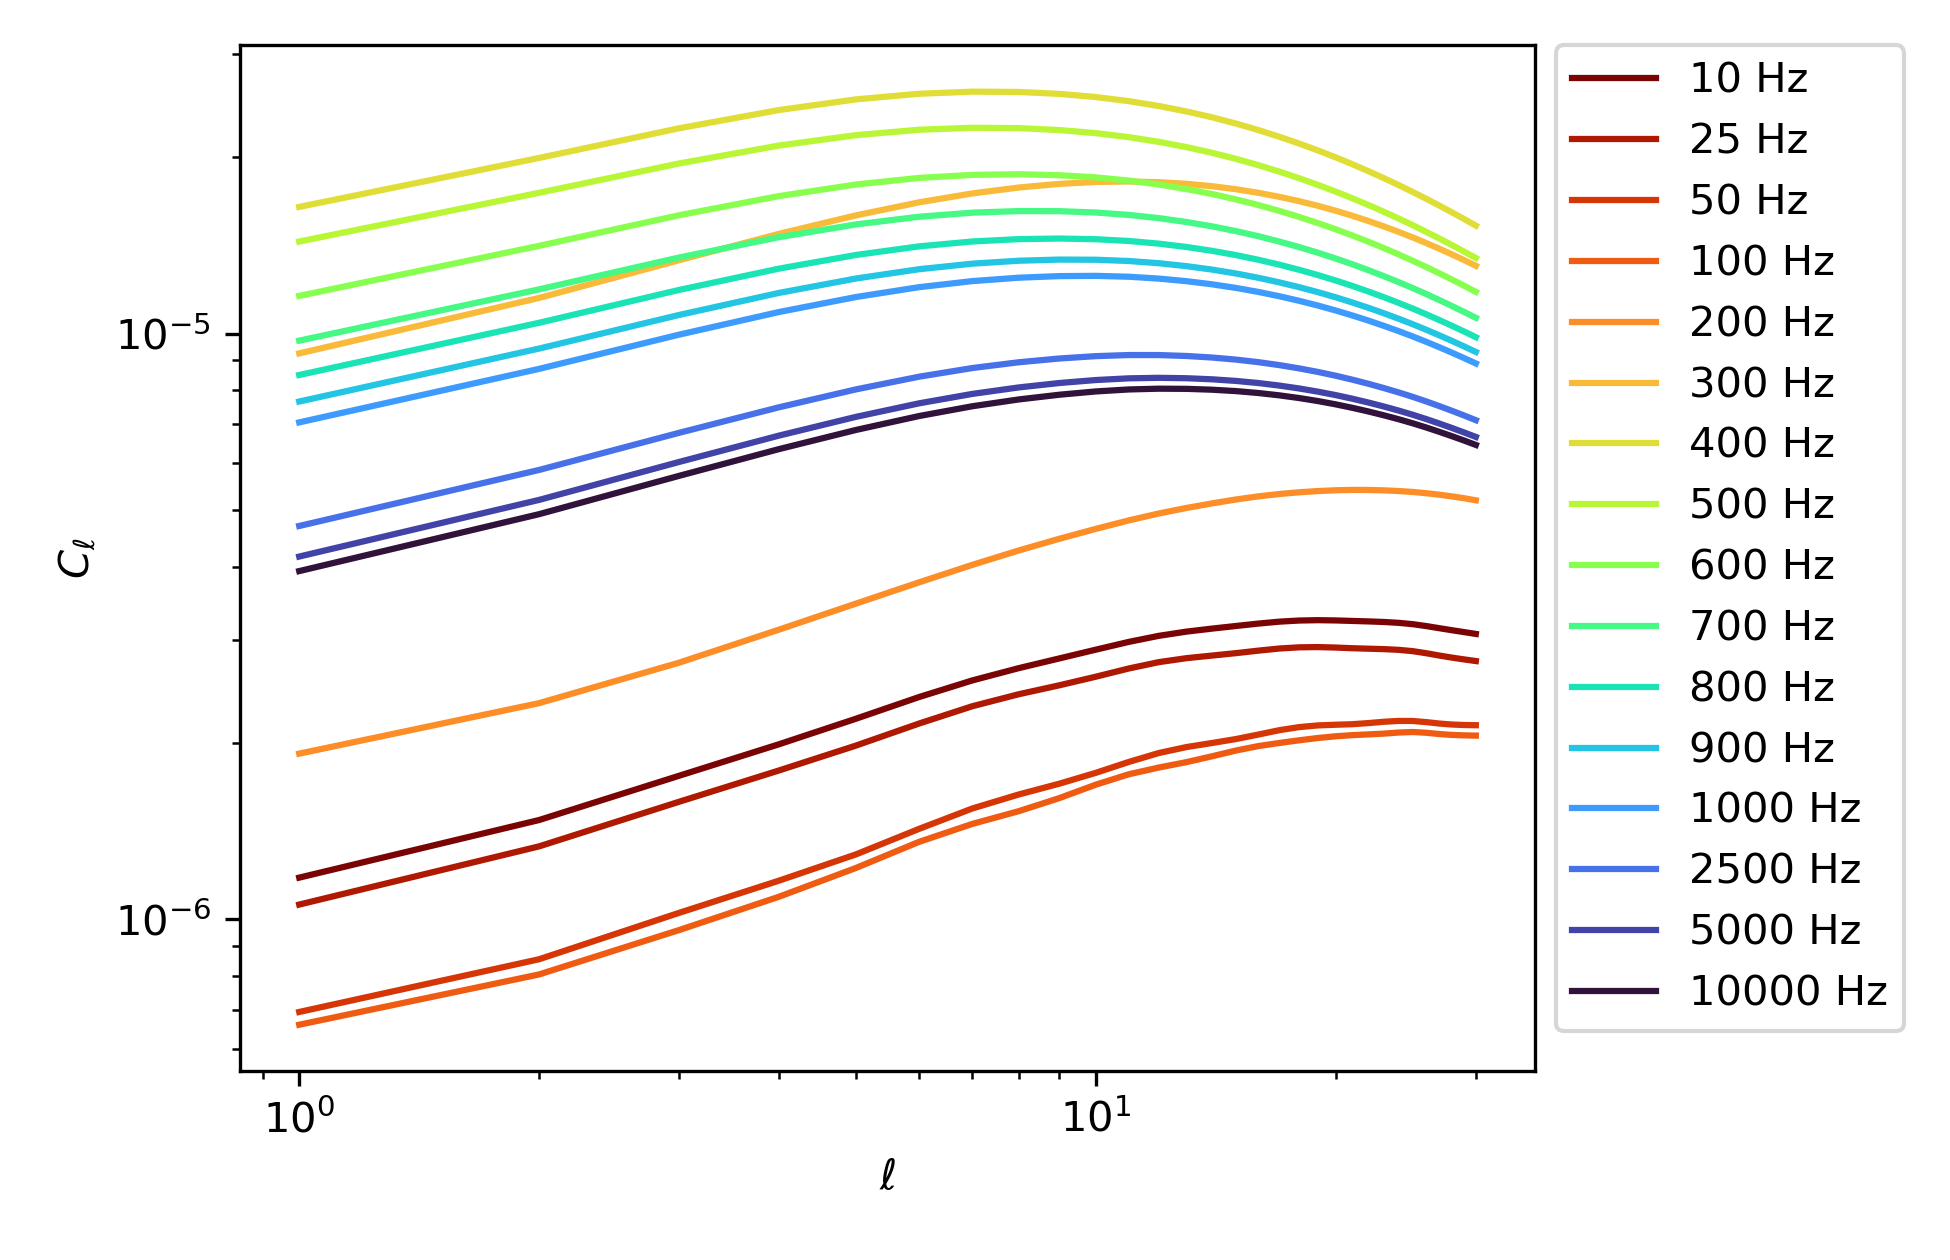
\includegraphics[width=1\linewidth]{Images/C_l_frequencies.png}
    \caption{AGWB angular power spectrum of different observed frequencies, going up to $l=30$.}
    \label{AGWB_anisotropies}
\end{figure} 

There is a clear frequency dependence of the angular power spectra ranging around one and a half orders of magnitude. We can see that the highest angular power spectrum occurs at 400 Hertz while the lowest is at 100 Hertz. If we focus on the dipole $l=1$, we can plot it as a function of frequency, see Fig.\ref{dipole_1000Hz}. The shape loosely resembles the energy spectrum in Fig. \ref{dE_df_f} which also peaks at around 400 Hertz and has a minimum at around 100 Hertz. the window function depends on frequency in through this energy spectrum multiplied by $f$ and divided by the monopole.

\begin{equation}
    \tilde{W}(z, f_o)\propto \frac{dE_{GW}/(df_e d\Omega_e)\;(f_e)}{\int dz (1+z)^{-1}H(z)^{-1}R_{BBH}(z) dE_{GW}/(df_e d\Omega_e)\;(f_e)}
\end{equation}

\begin{figure}
    \centering
    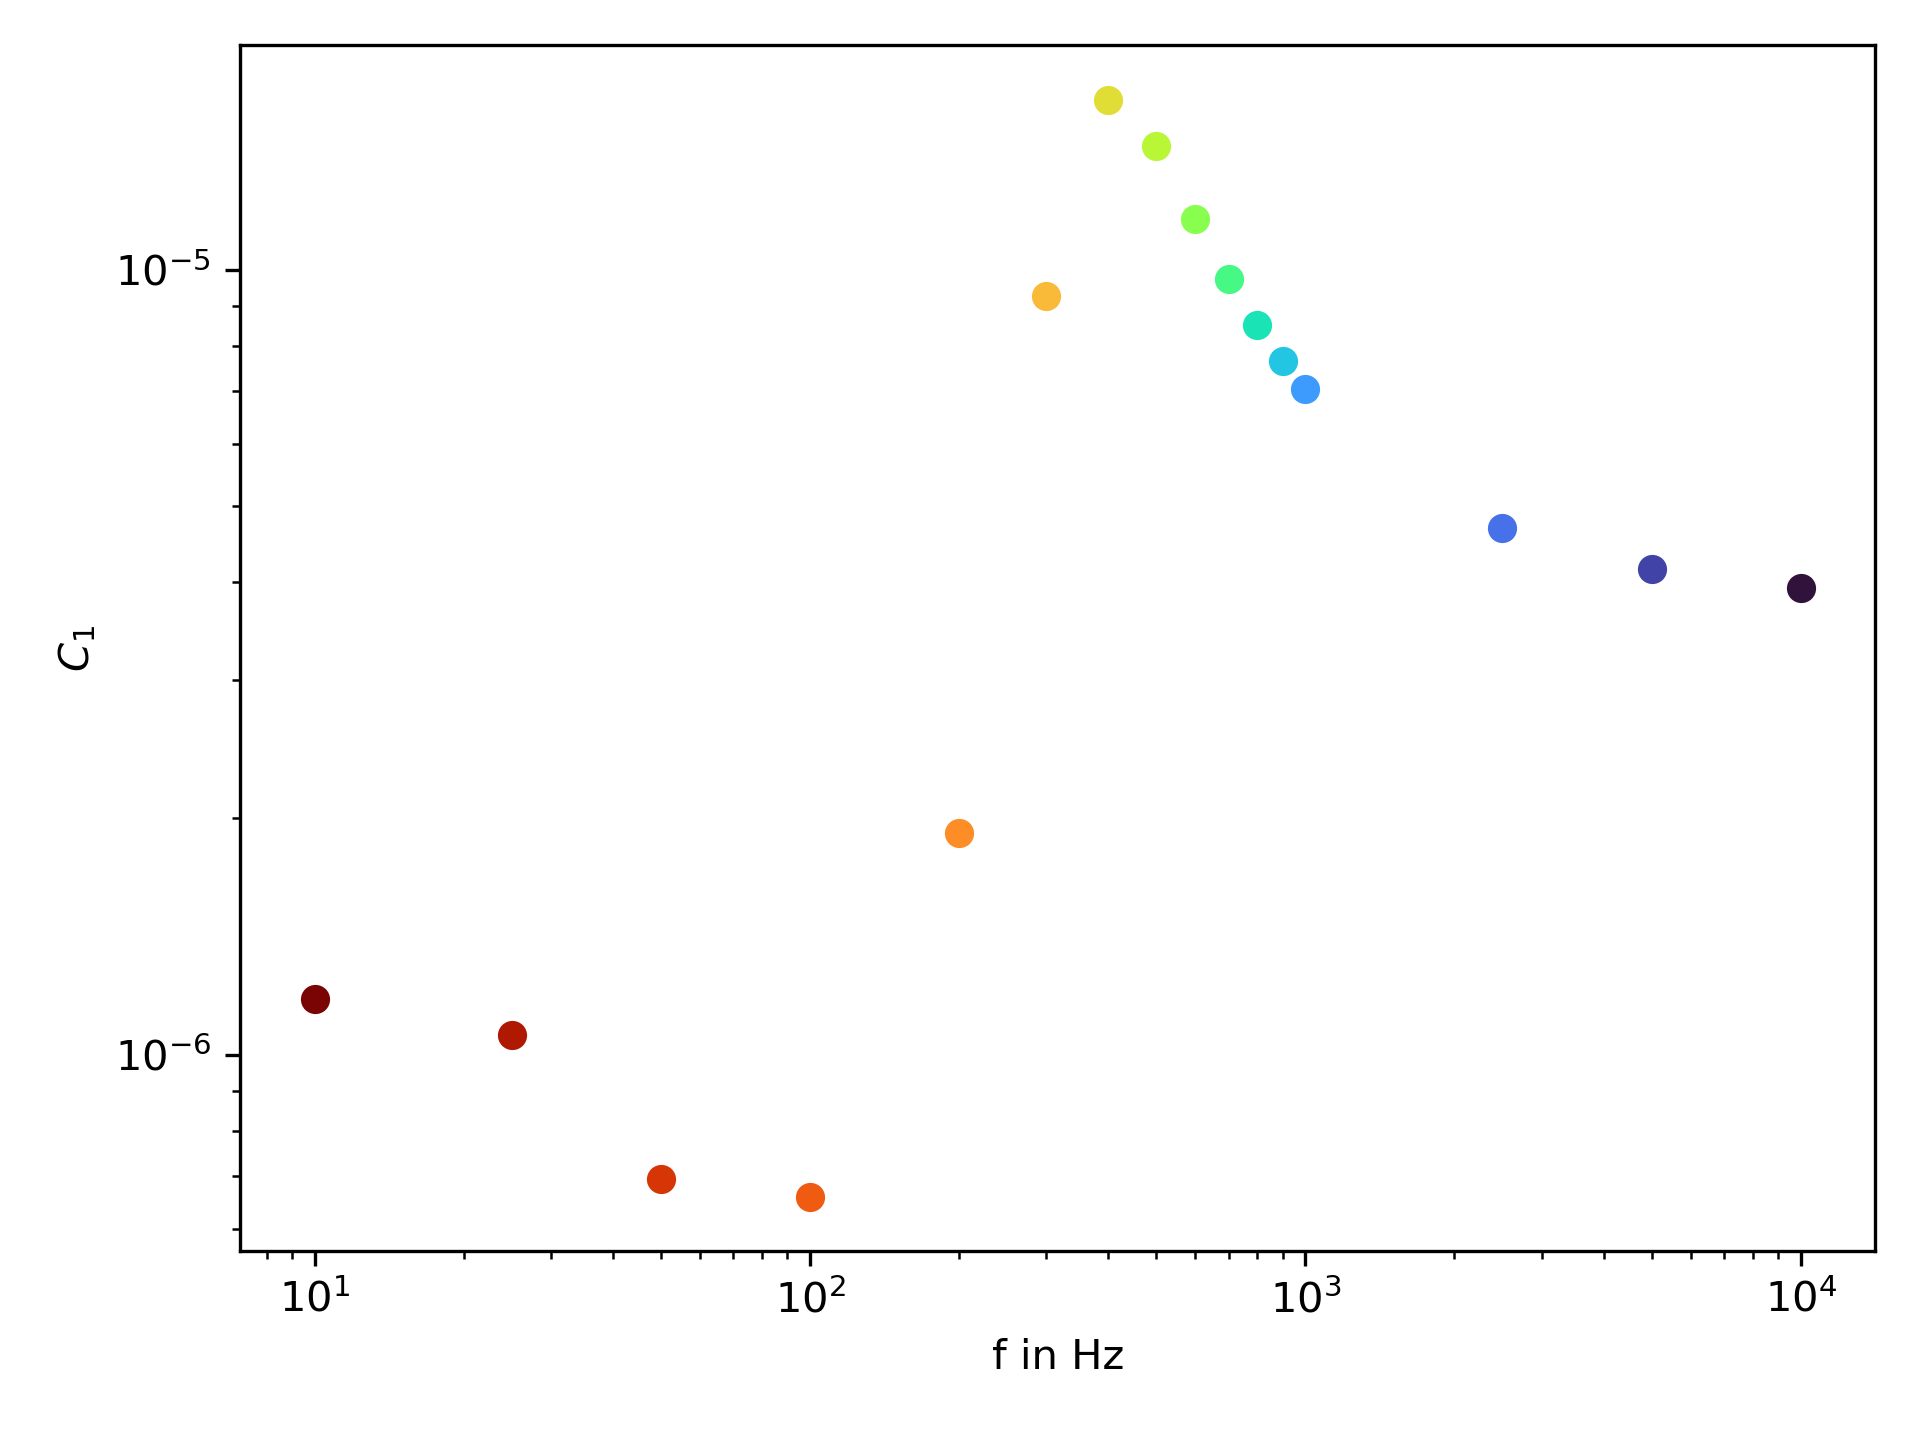
\includegraphics[width=0.8\linewidth]{Images/dipole_frequencies_10000Hz.png}
    \caption{The dipole of the AGWB at different observed frequencies.}
    \label{dipole_1000Hz}
\end{figure} 

To compare our results, we use \cite{dallarmi_dipole_2022} and their frequency-dependent dipole in Fig. \ref{lorenzo_comparison}. They additionally computed the kinematic dipole coming from our observer velocity with respect to the rest frame of the large scale structure. Furthermore, they considered the shot noise. This is the variance from a Poisson distribution which the GW mergers follow. We compare our intrinsic anisotropies with theirs in blue. The rough shape of our calculation looks similar, reaching a minimum at $\approx 100$ Hertz, then peaking and declining again. In their plot, the peak is at $\approx 200$ Hertz which is a lower frequency than ours. Additionally, they observe a continuous exponential increase (due to the lin-log axes) for frequencies above $\approx 400$ Hertz. In this work this increase is not present. Even at higher frequencies up to 10,000 Hertz (see Fig. \ref{dipole_1000Hz}) the dipole does not increase. Physically, higher frequencies correspond to a higher chirp mass $M_c$, so a binary with higher masses.

\begin{figure}
    \centering
    \subfloat[{This work}
        \label{lorenzo_dipole}]{
        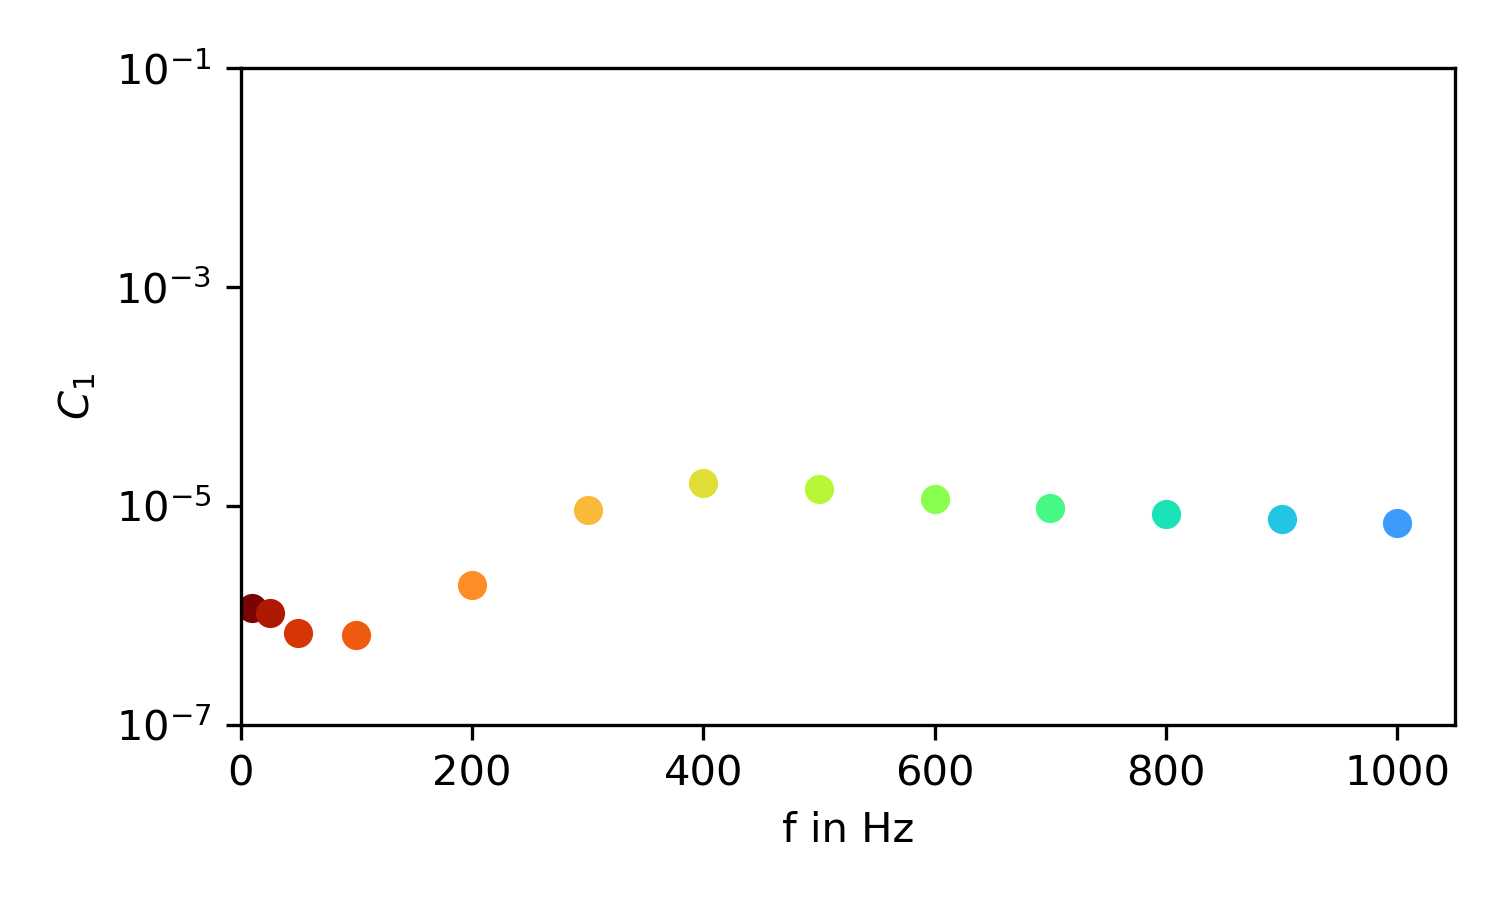
\includegraphics[width=8cm, clip]{Images/dipole_frequencies.png}}
    \subfloat[{\cite{dallarmi_dipole_2022}}
        \label{dipole_1000Hz}]{
        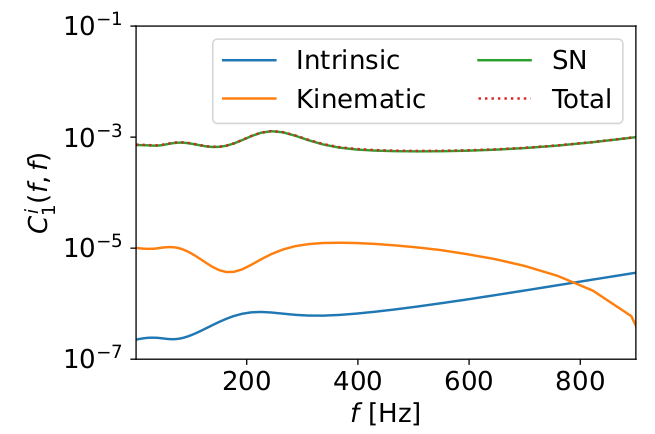
\includegraphics[width=7cm, clip]{Images/lorenzo_dipole.png}}
    \caption[Comparison of the computed dipole contribution to \cite{dallarmi_dipole_2022}.]{Comparison of the computed dipole contribution. On the left are the computed anisotropies using our formalism for the intrinsic anisotropies. On the right, the computed dipole by \cite{dallarmi_dipole_2022}. The intrinsic dipole is shown in blue, the kinematic dipole in orange and the shot noise for the dipole in green.}
    \label{lorenzo_comparison}
\end{figure} 


\section{AGWB vs. Noise}

To compare to the noise levels in section \ref{ET_CE}, we have to keep in mind that we calculated relative $C_l$ with respect to the monopole. This is because we start with the density contrast in section \ref{window_fct_section}.

\begin{equation}
    \delta_{AGWB}(f_o, \hat{n})=\frac{\Omega_{AGWB}(f_o, \hat{n})-\bar{\Omega}_{AGWB}(f_o)}{\bar{\Omega}_{AGWB}(f_o)}
\end{equation}
\begin{equation}
    =\int dz \tilde{W}(f_0, z)\Delta_{AGWB}(f_0, \hat{n}, z)
\end{equation}

Since the anisotropies are a two-point correlation, they depend quadratically on the source functions which come from the density contrast above.

\begin{equation}
    C_l = 4\pi \int \frac{dk}{k} P(k) \Delta_l \Delta_l^*
\end{equation}

Thus, to compute the physical angular power spectrum, we need to divide by the squared monopole over the solid angle.

\begin{equation}
    C_l^{rel}=C_l \frac{(4\pi)^2}{\bar{\Omega}_{GW}^2}
\end{equation}
\begin{figure}[h]
    \centering
    \subfloat{\hspace{1cm}
        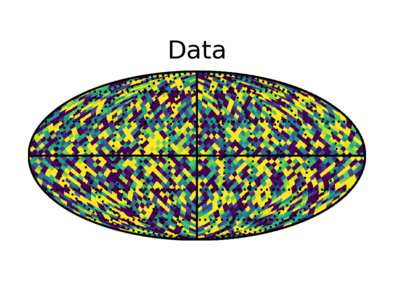
\includegraphics[width=5cm]{Images/data_100Hz_2D.png}
        }
    \newline
    \vspace{-1.5cm}
    \subfloat{
        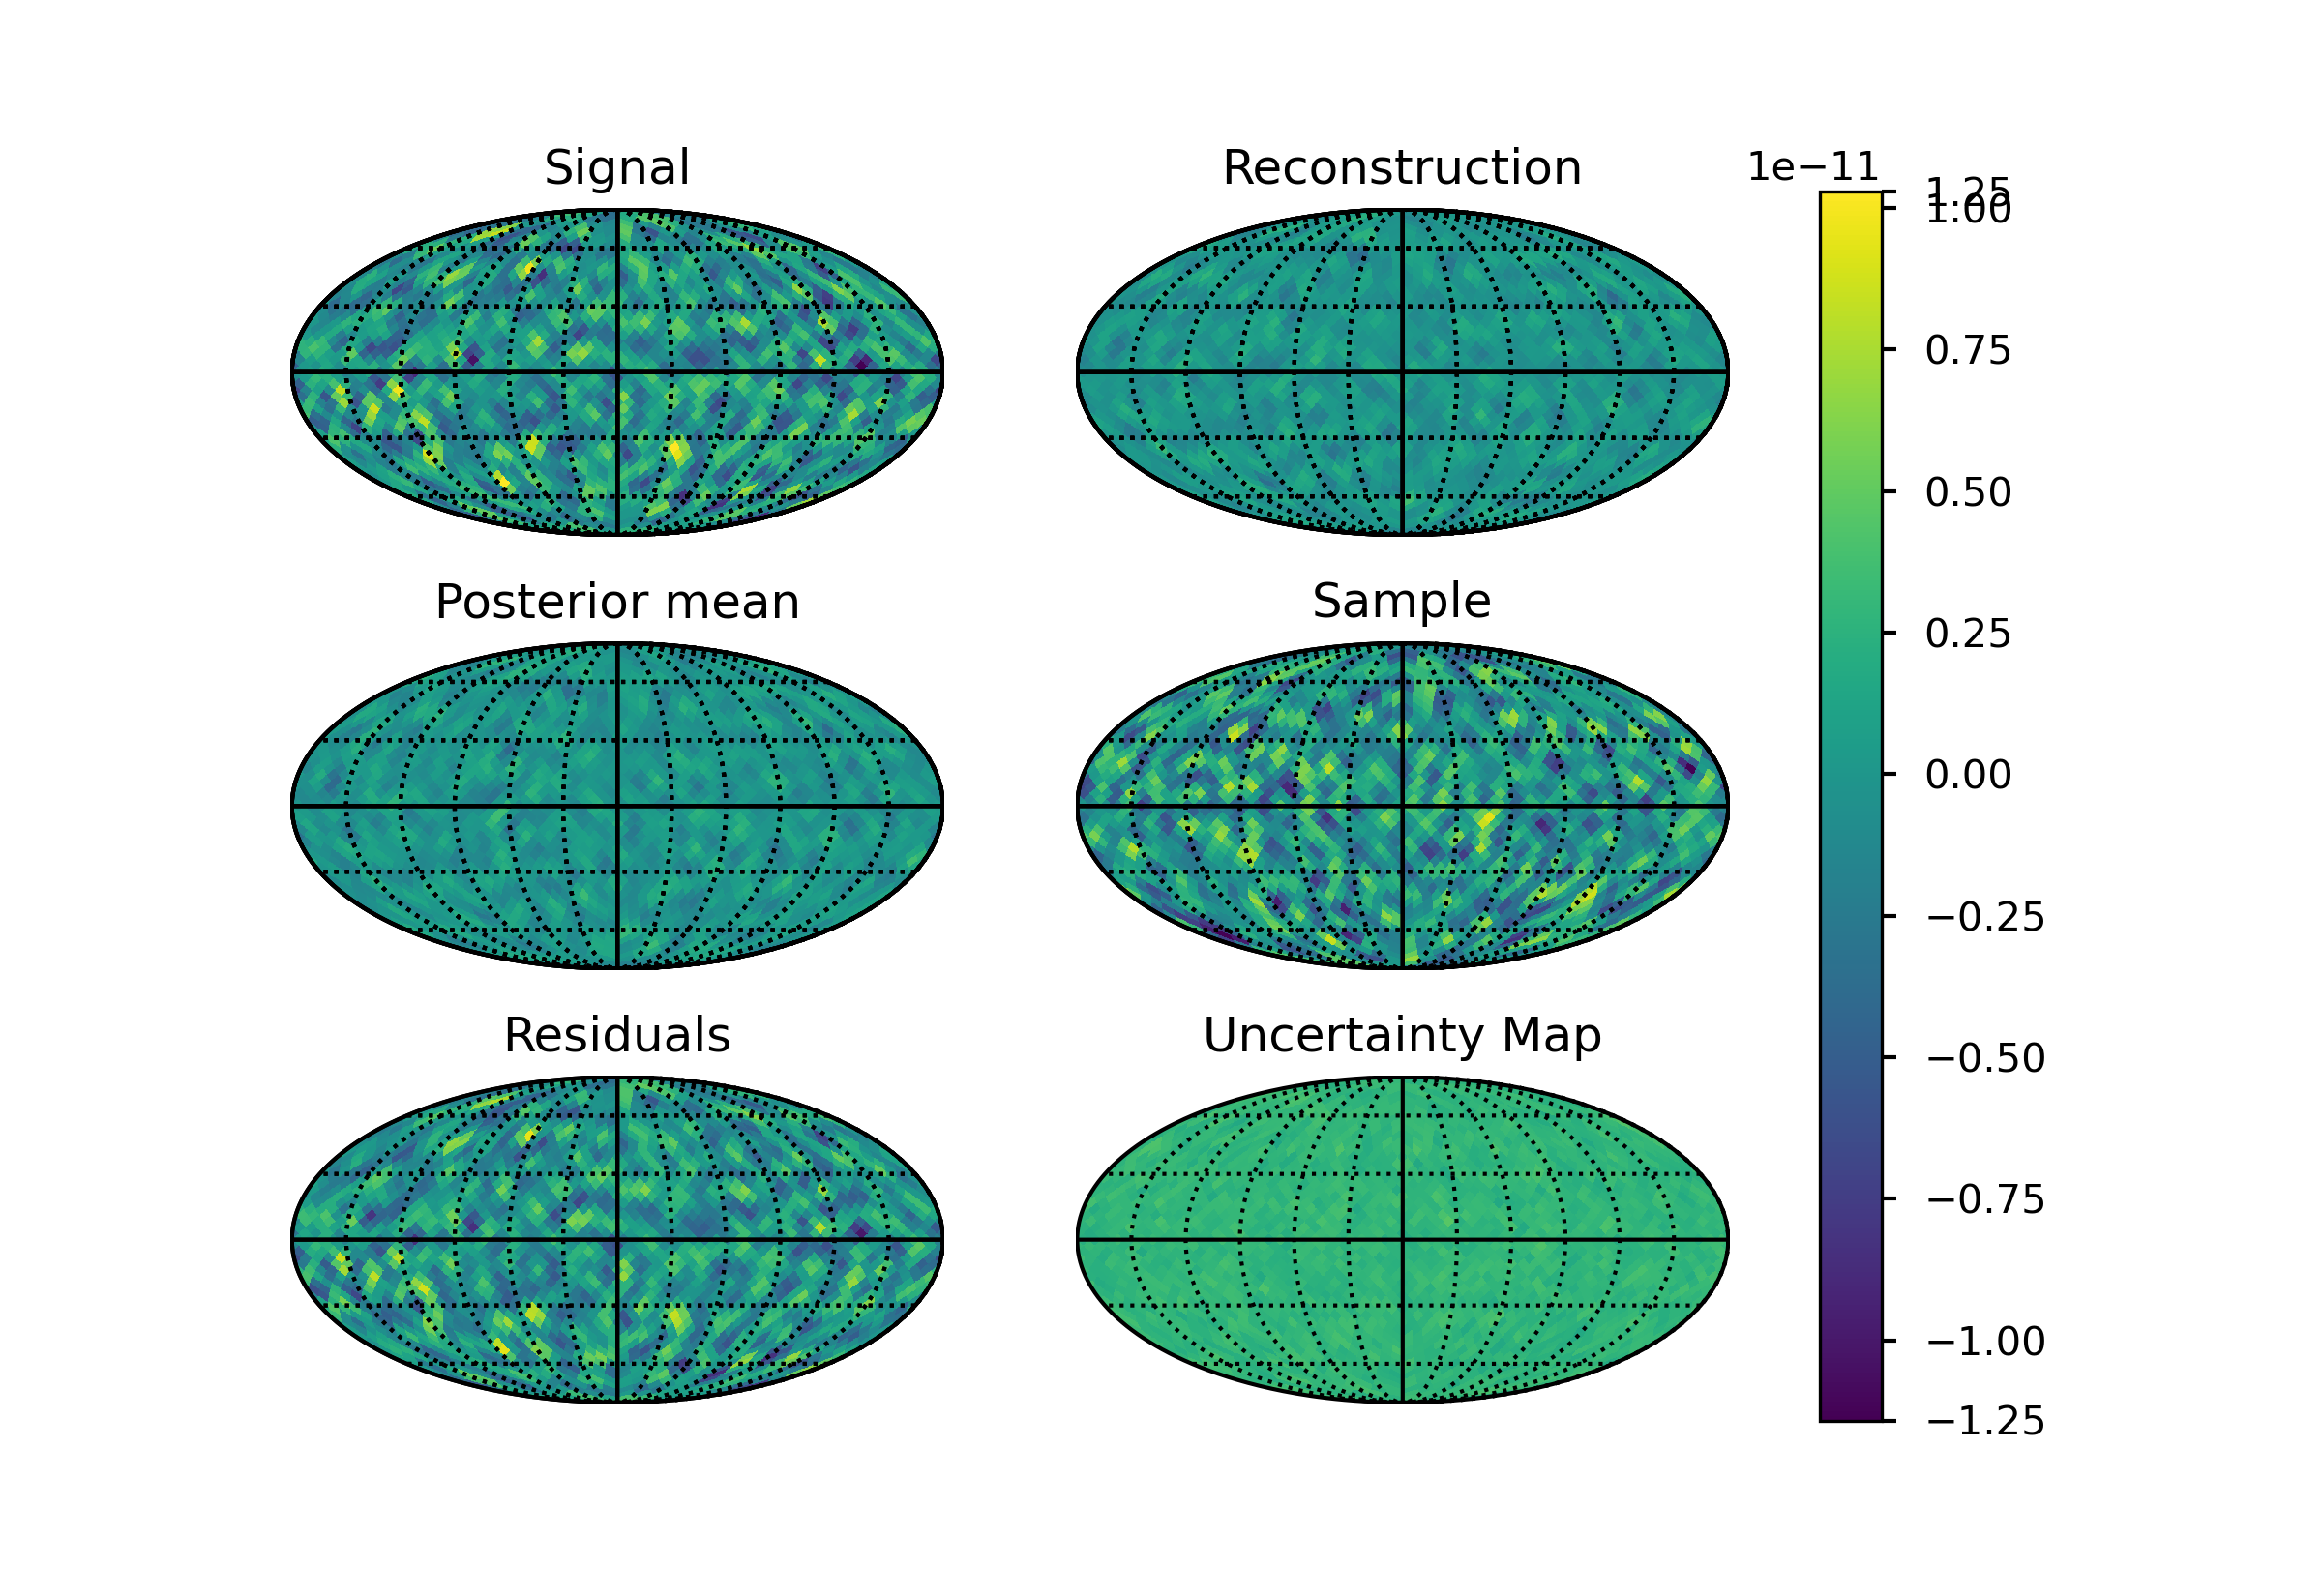
\includegraphics[width=\linewidth]{Images/6plot_100Hz_2D.png}}
    \caption[Reconstruction of the AGWB at 100 Hertz on a sky map using the {\tt NIFTy} code.]{Reconstruction of the AGWB at 100 Hertz on a sky map using the {\tt NIFTy} code. The data on top is generated from the signal which is a realisation of the input power spectrum. The posterior mean is calculated using a Wiener filter. A sample of this is drawn randomly. The residuals represent the difference between signal and reconstruction from the first row. The uncertainty map shows the calculated errors on the reconstruction.}
    \label{sky_maps_100}
\end{figure}

\begin{figure}
    \centering
    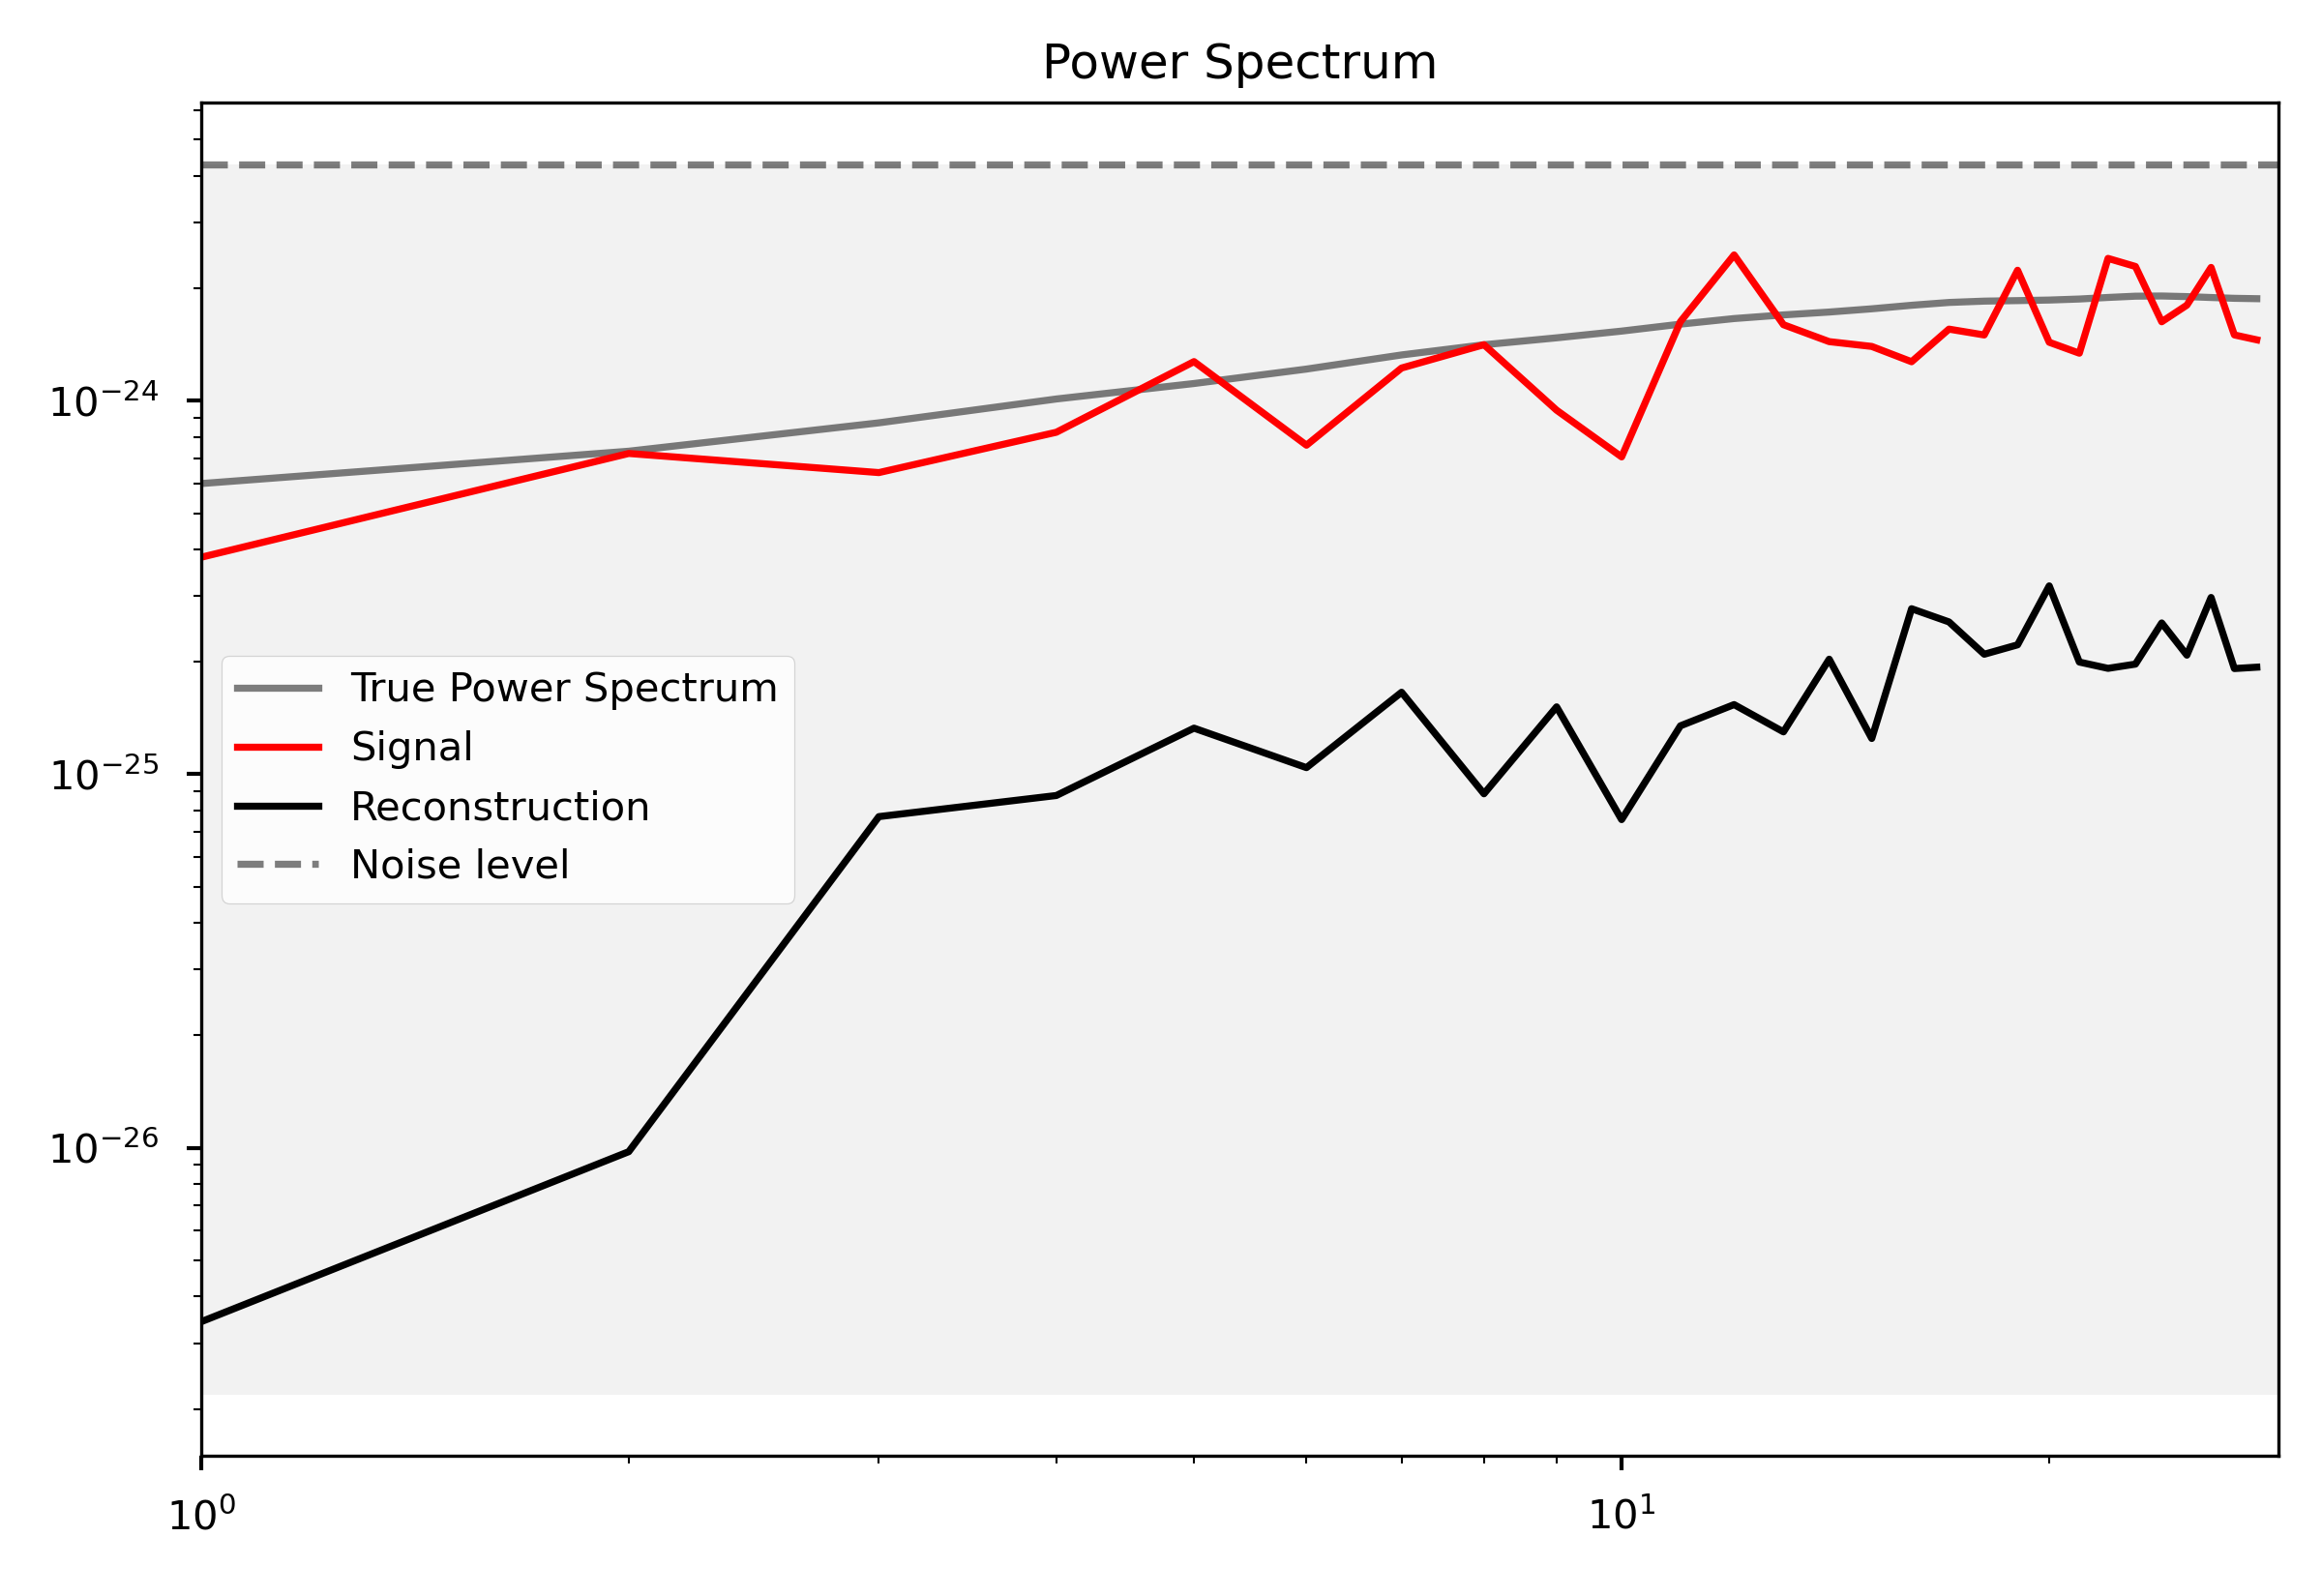
\includegraphics[width=0.8\linewidth]{Images/power_spectrum_100Hz_2D.png}
    \caption[The power spectra of the AGWB separation at 100 Hertz.]{The power spectra of the AGWB separation at 100 Hertz. The input power spectrum is shown in grey, the signal realisation in red and the reconstruction using IFT in black.}
    \label{100Hz_power_spectrum}
\end{figure} 

For the noise angular power spectrum, we assume Gaussian noise using the best anisotropic noise sensitivity for ET and CE using cross-correlations (at $l=1$). This is an optimistic assumption. The computed $C_l$ used for the separation reach up to $l=30$. Looking at Fig. \ref{ET_Cl}, our assumed noise curve would have the shape of $l+\frac{1}{2}$ up to $l=30$, which would increase more slowly than the actual sensitivity curve. 

As seen in Fig.\ref{AGWB_anisotropies}, we compute the lowest angular power spectrum at a frequency of 100 Hertz. To test the separation in this case, we use it as input for a reconstruction on a sky map using {\tt HEALPix}\cite{todo, healpix}. At this frequency, the separation is not successful. We see that the noise in the data in Fig.\ref{sky_maps_100} is higher than the original signal. The posterior mean and the reconstruction are both close to zero. Thus, the sample also does not mimic the signal and the residuals have the same order of magnitude as the original signal.

In the power spectrum in Fig. \ref{100Hz_power_spectrum}, we can see that the noise is roughly one order of magnitude higher than the input power spectrum which explains why a separation is not possible. The reconstruction is much lower. By trying to filter out the noise, the signal gets filtered out as well in this case. To successfully separate the signal at 100 Hertz, we would need a detector that is around 2 orders of magnitude better in sensitivity compared to ET+CE.

The AGWB has the highest angular power spectrum at 400 Hertz in our calculation (see Fig.\ref{AGWB_anisotropies}). So, we use this frequency to perform another IFT separation. In the separation in Fig. \ref{sky_maps_400}, the data resembles the signal more closely than for 100 Hertz. Comparing the signal to the reconstruction sky map, we see that most maxima and minima are recovered successfully. The posterior mean from the Wiener filter also mimics the signal map. When a sample is drawn from this posterior, it has some more pronounced minima and maxima but still follows the signal. However, our residuals have the same order of magnitude as the signal which is reflected in the uncertainty map as well.

\begin{figure}[h]
    \centering
    \subfloat{\hspace{1cm}
        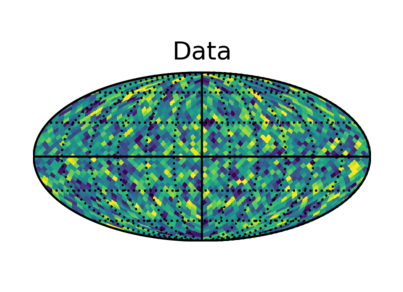
\includegraphics[width=5cm]{Images/data_400Hz_2D.png}
        }
    \newline
    \vspace{-1.5cm}
    \subfloat{
        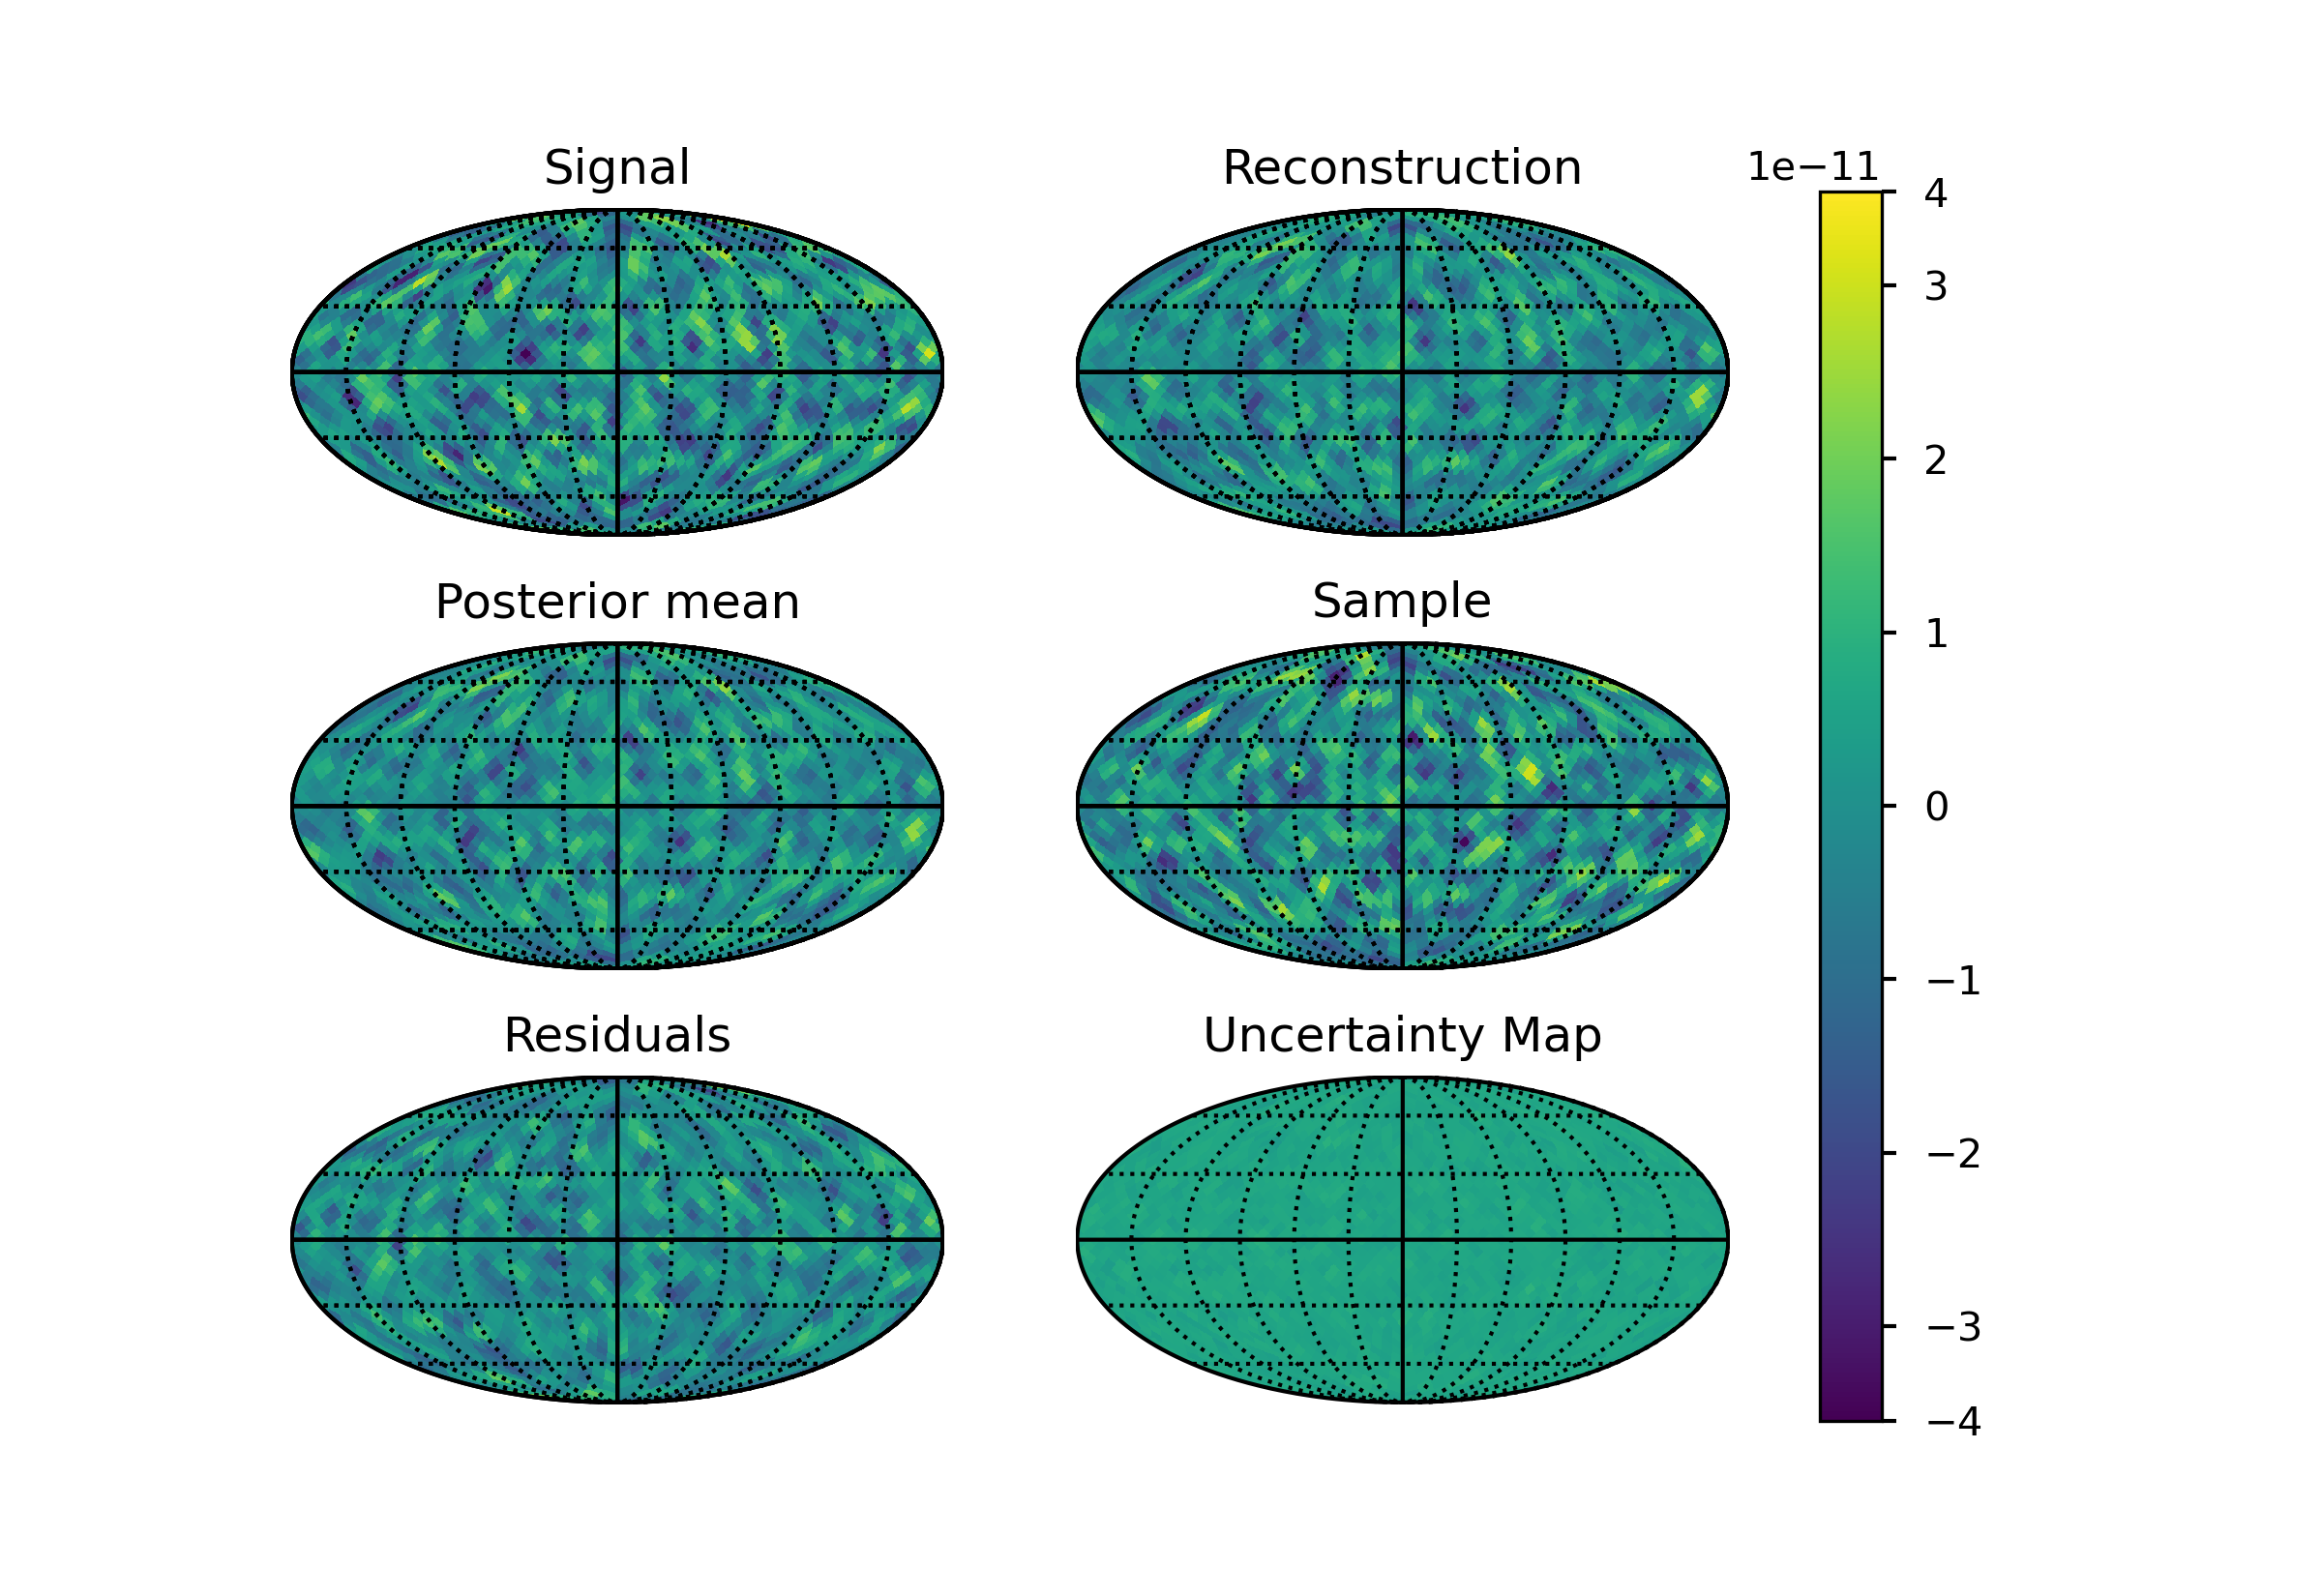
\includegraphics[width=\linewidth]{Images/6plot_400Hz_2D.png}}
    \caption[Reconstruction of the AGWB at 400 Hertz on a sky map using the {\tt NIFTy} code.]{Reconstruction of the AGWB at 400 Hertz on a sky map using the {\tt NIFTy} code. The data on top is generated from the signal which is a realisation of the input power spectrum. The posterior mean is calculated using a Wiener filter. A sample of this is drawn randomly. The residuals represent the difference between signal and reconstruction from the first row. The uncertainty map shows the calculated errors on the reconstruction.}
    \label{sky_maps_400}
\end{figure}

In this case, the noise is half an order of magnitude lower than our power spectrum at 400 Hertz which is why the reconstruction is relatively successful, see Fig. \ref{400Hz_power_spectrum}. Regardless, the reconstruction is lower at all scales compared to the signal. If the detectors had a sensitivity of half or one order of magnitude lower, this reconstruction would be very feasible at 400 Hertz.

\begin{figure}[h]
    \centering
    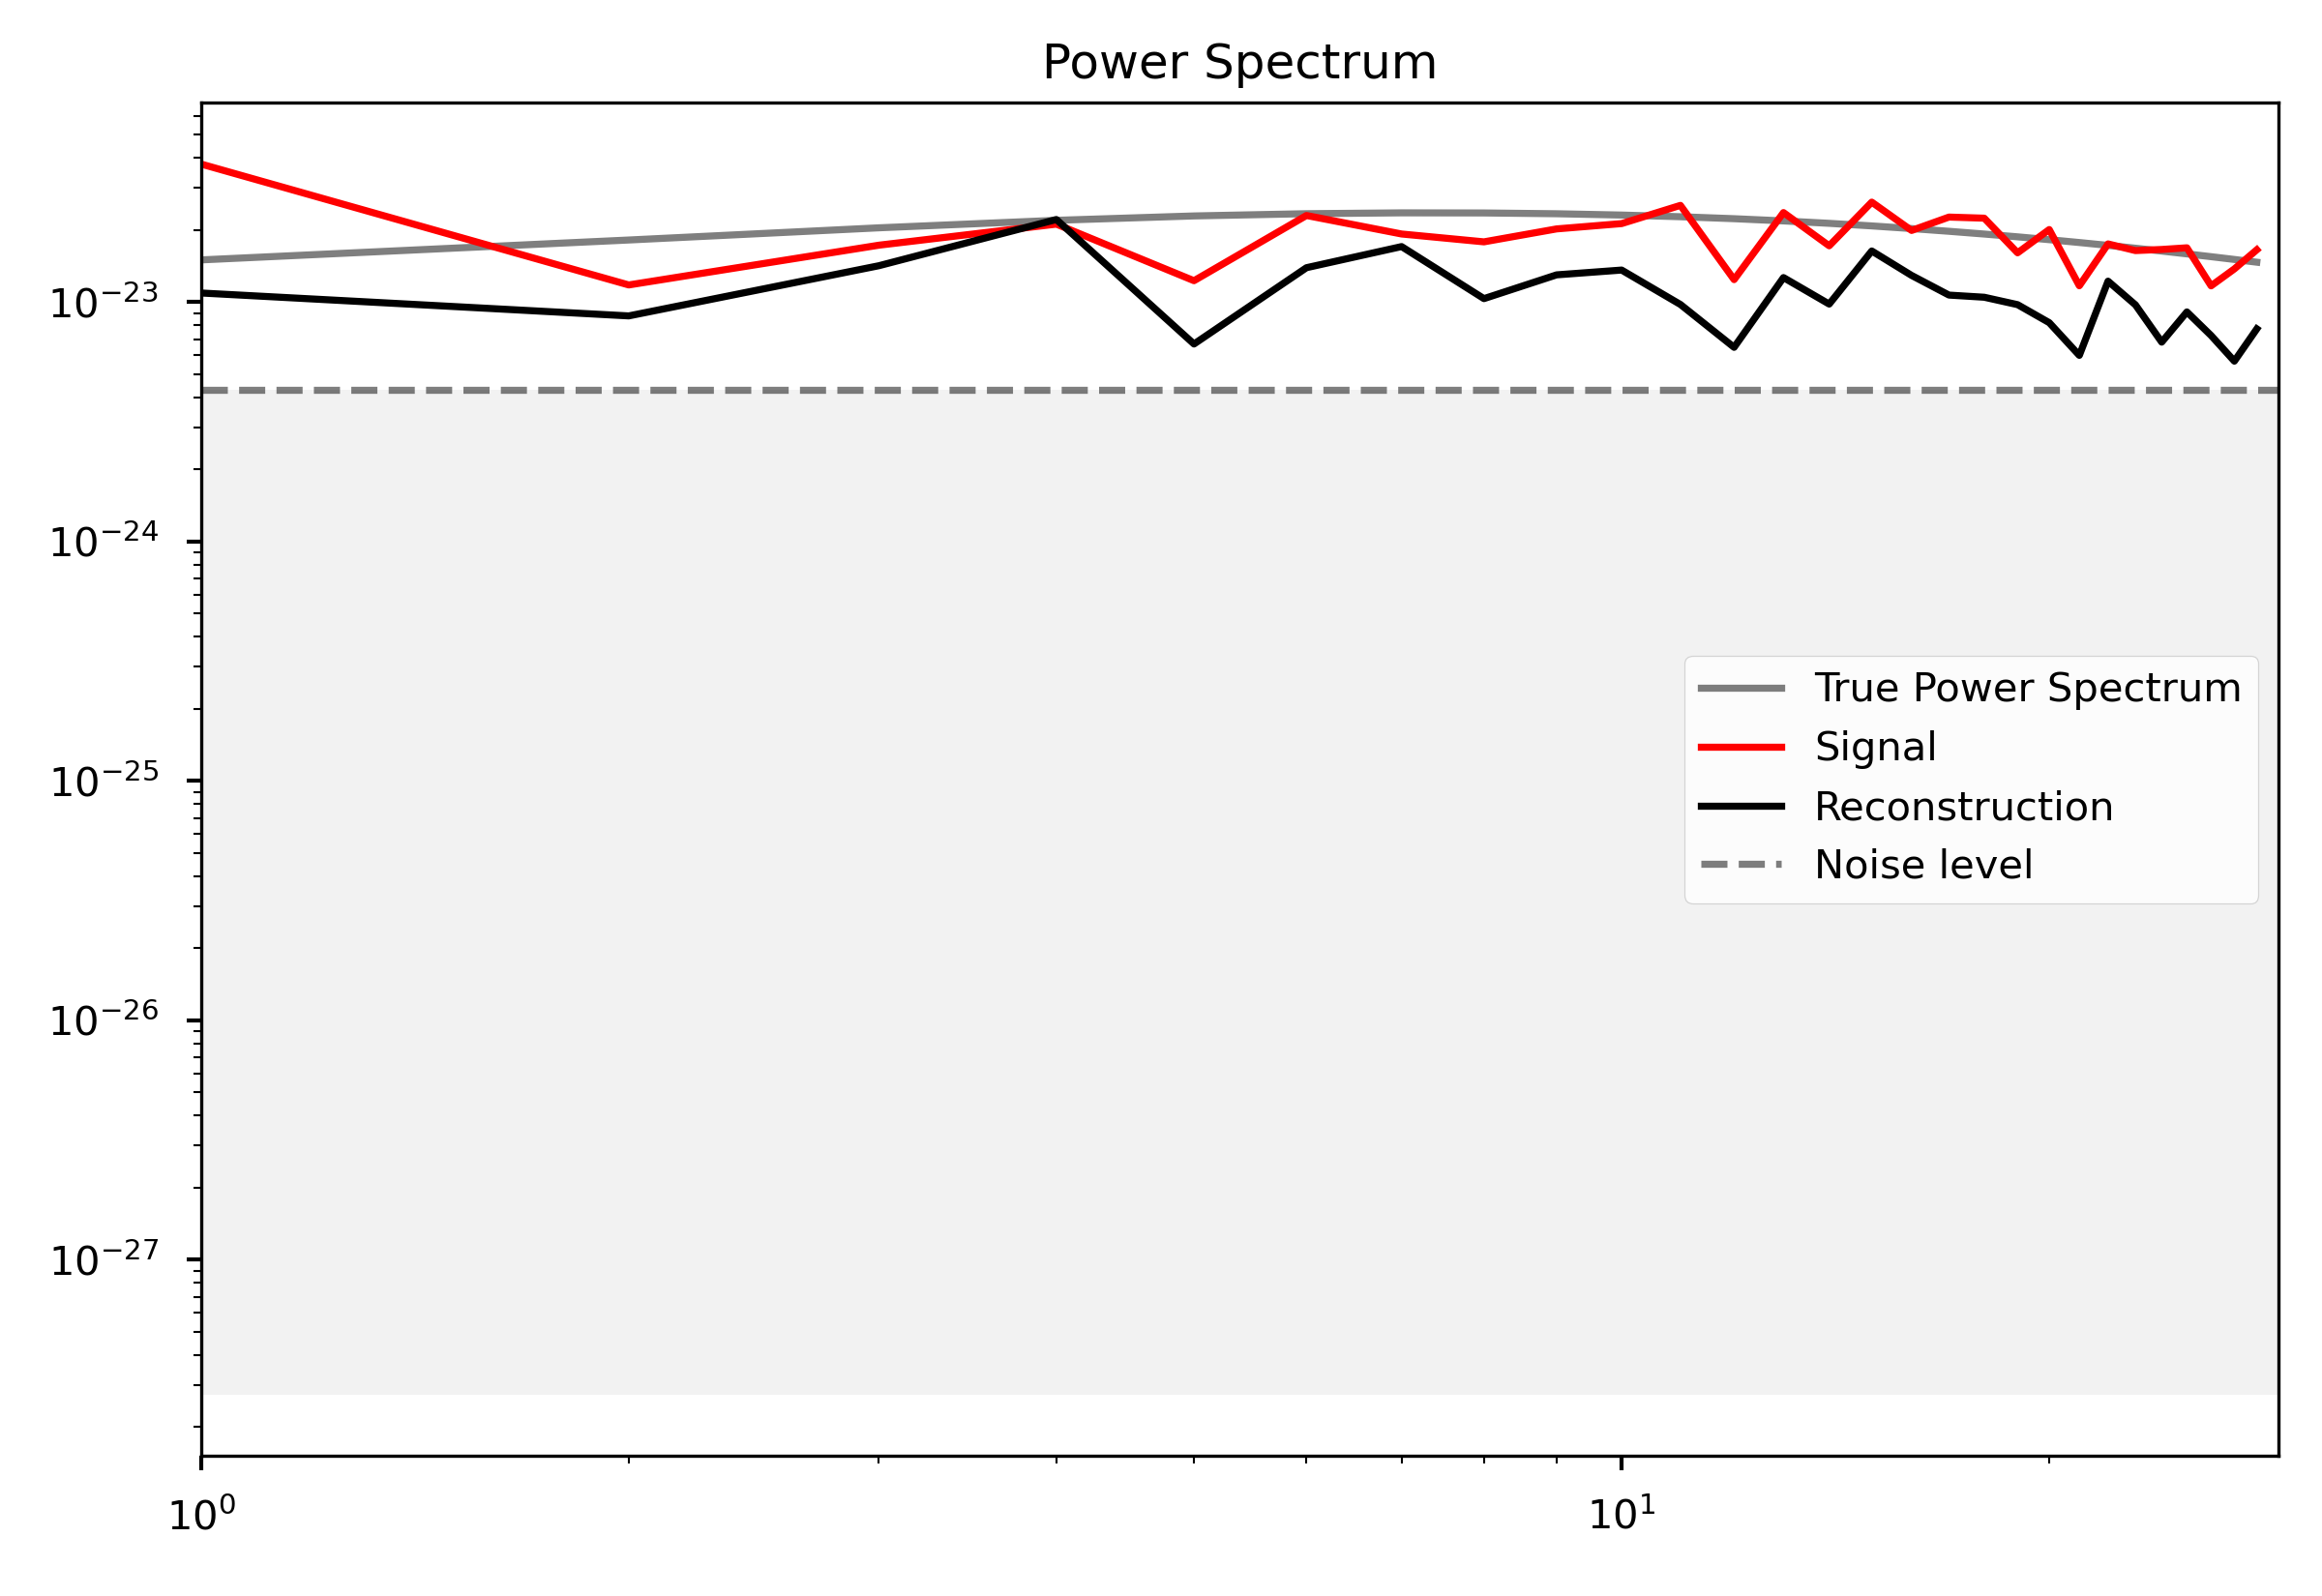
\includegraphics[width=0.8\linewidth]{Images/power_spectrum_400Hz_2D.png}
    \caption[The power spectra of the AGWB separation at 400 Hertz.]{The power spectra of the AGWB separation at 400 Hertz. The input power spectrum is shown in grey, the signal realisation in red and the reconstruction using IFT in black.}
    \label{400Hz_power_spectrum}
\end{figure} 

\section{CGWB vs. Noise}

Ideally, we could also detect the cosmological GW background with future experiments. To see how feasible this is, we use the {\tt GW\_CLASS} code by \cite{schulze_gw_class_2023} that is also based on {\tt CLASS}. 
\begin{figure}[h]
    \centering
    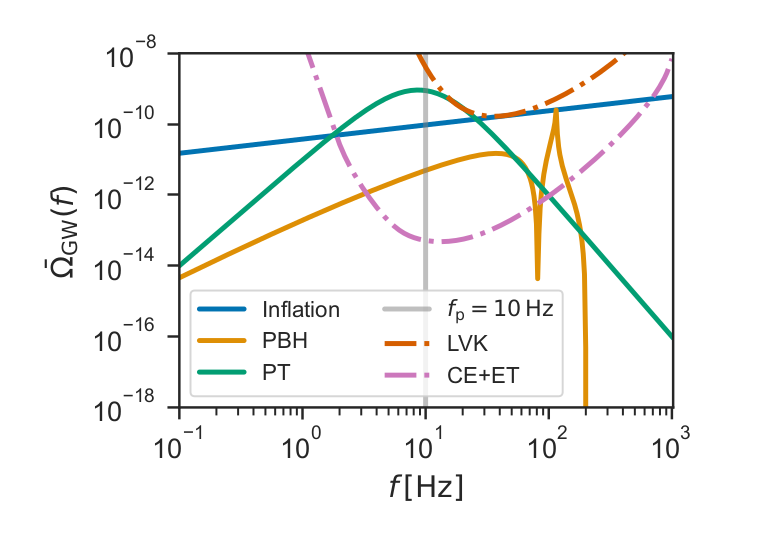
\includegraphics[width=0.6\linewidth]{Images/schulze_monopole.png}
    \caption[Frequency dependence of the monopole of the cosmological GW background for different generation mechanisms.]{Frequency dependence of the monopole of the cosmological GW background for different generation mechanisms. The inflation scenario is shown in blue, primordial BH in orange and GW from phase transitions in green. The sensitivities for LVK and ET+CE are also shown for the monopole background.}
    \label{cosmo_monopole}
\end{figure} 

We assume a cosmological GW background coming only from inflation, see section \ref{cosmo_bg}. This has a blue tilt, meaning the background increases with frequency. To see the frequency dependency, we can look at the monopole amplitude shown in Fig.\ref{cosmo_monopole}.



\begin{figure}[h]
    \centering
    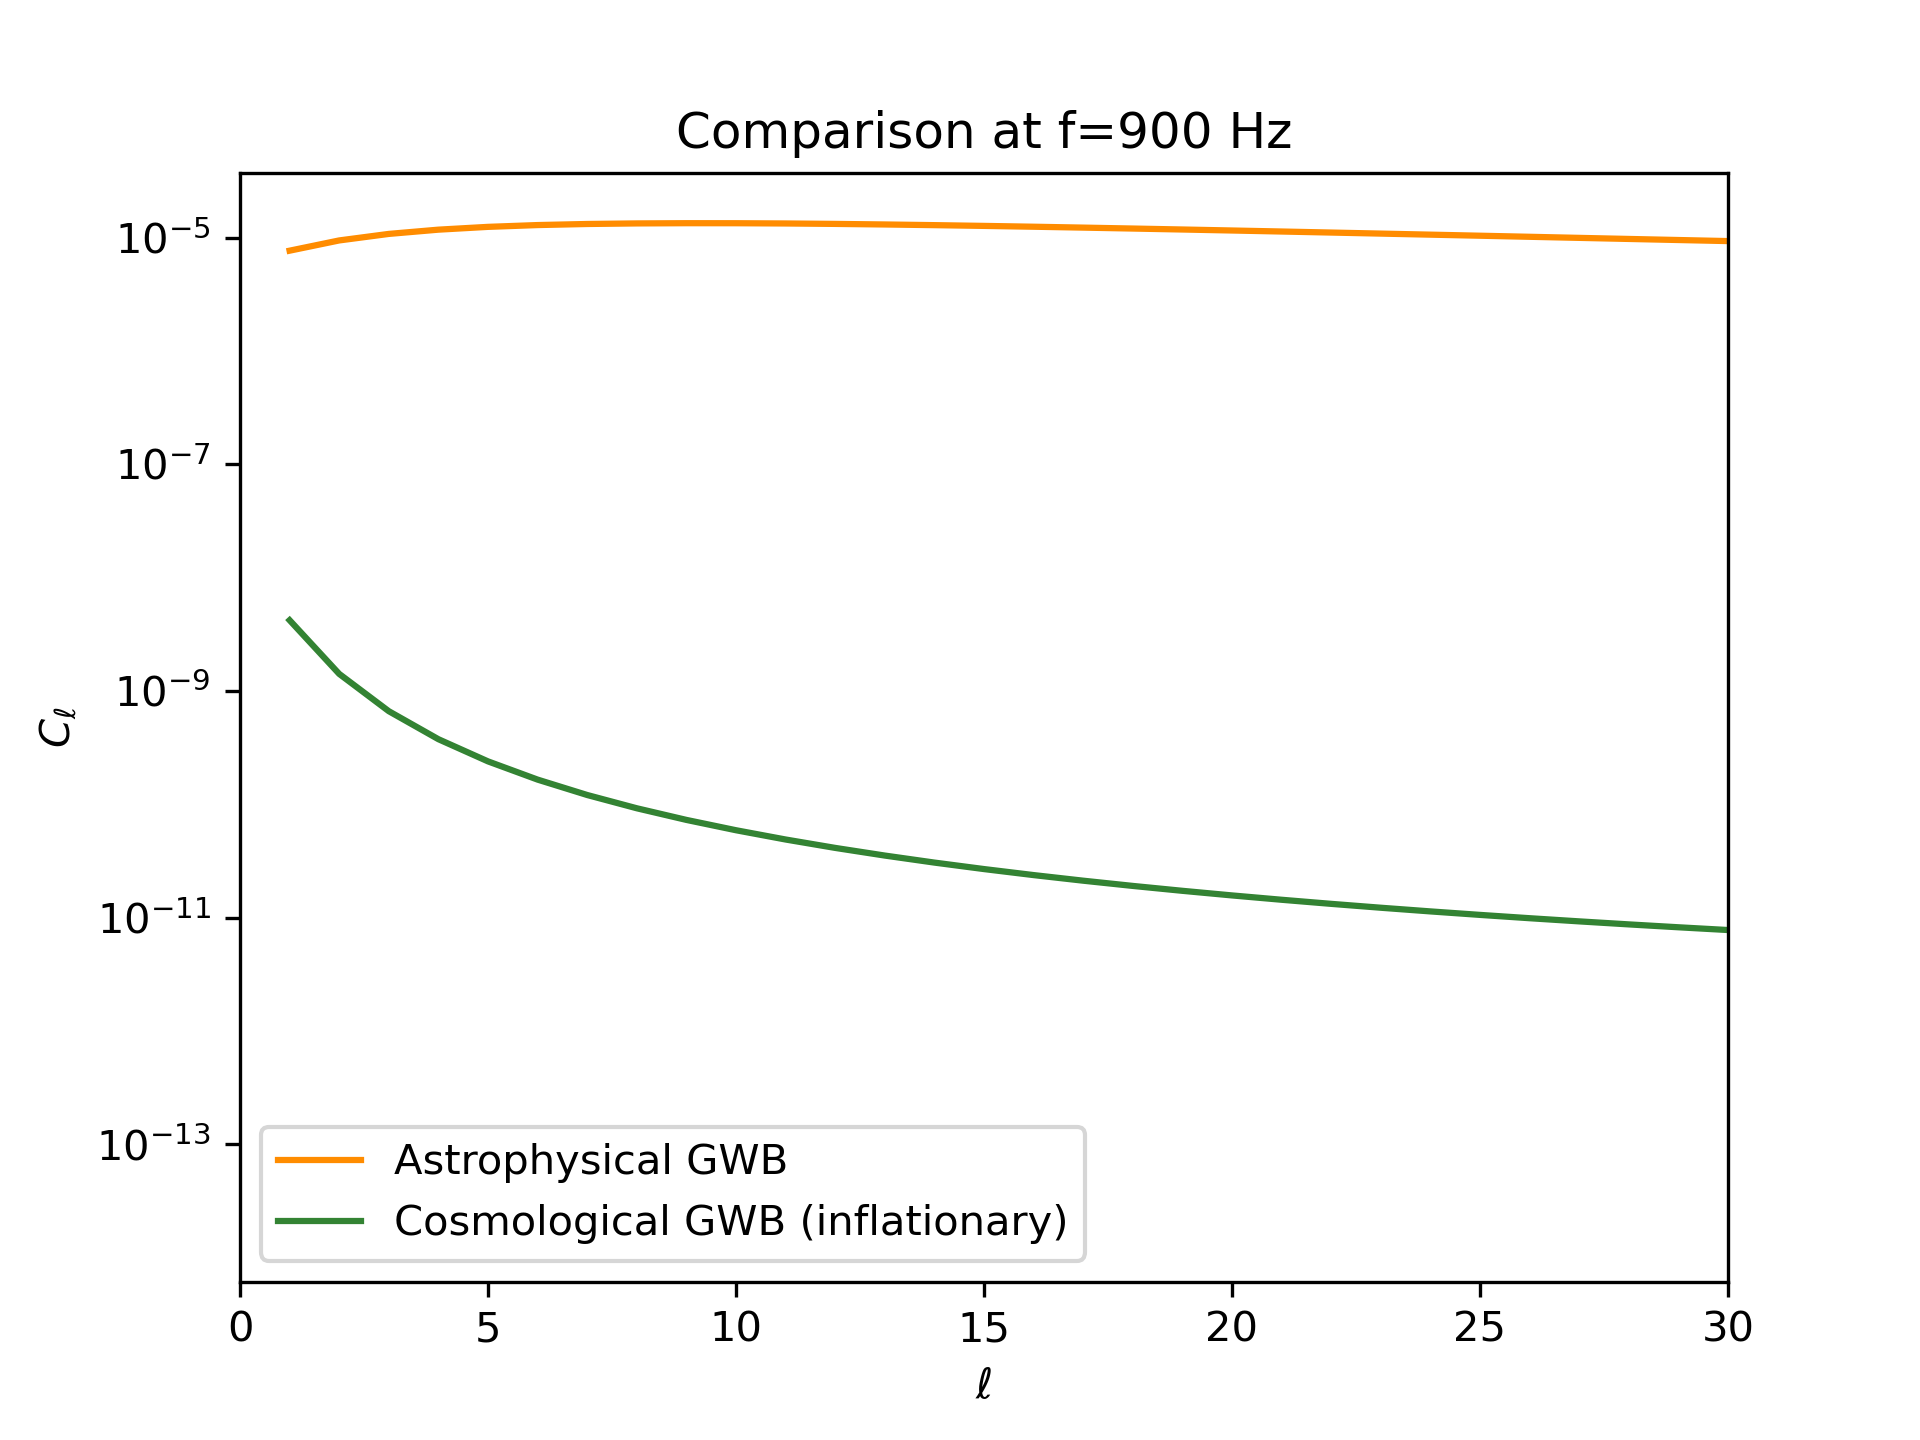
\includegraphics[width=0.6\linewidth]{Images/astro_vs_cosmo.png}
    \caption{A comparison of the angular power spectra of the astrophysical versus the inflationary cosmological GW background at 900 Hertz.}
    \label{astro_cosmo}
\end{figure} 

Due to the blue tilt, we use a high frequency of 900 Hertz to test the IFT separation.
We can compare this to the AGWB at the same frequency, see Fig.\ref{astro_cosmo}. The AGWB is two to three orders of magnitude higher depending on the multipole. 


The assumed noise is the same as for the AGWB case. Again, the relative $C_\ell$ are converted into physical $C_\ell$.

\begin{figure}[h]
    \centering
    \subfloat{\hspace{1cm}
        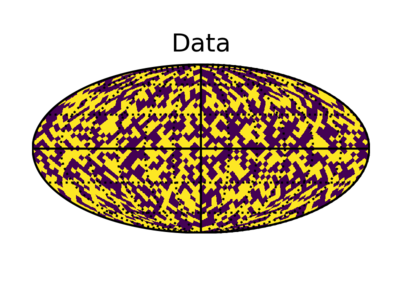
\includegraphics[width=5cm]{Images/data_cosmo_900Hz_2D.png}
        }
    \newline
    \vspace{-1.5cm}
    \subfloat{
        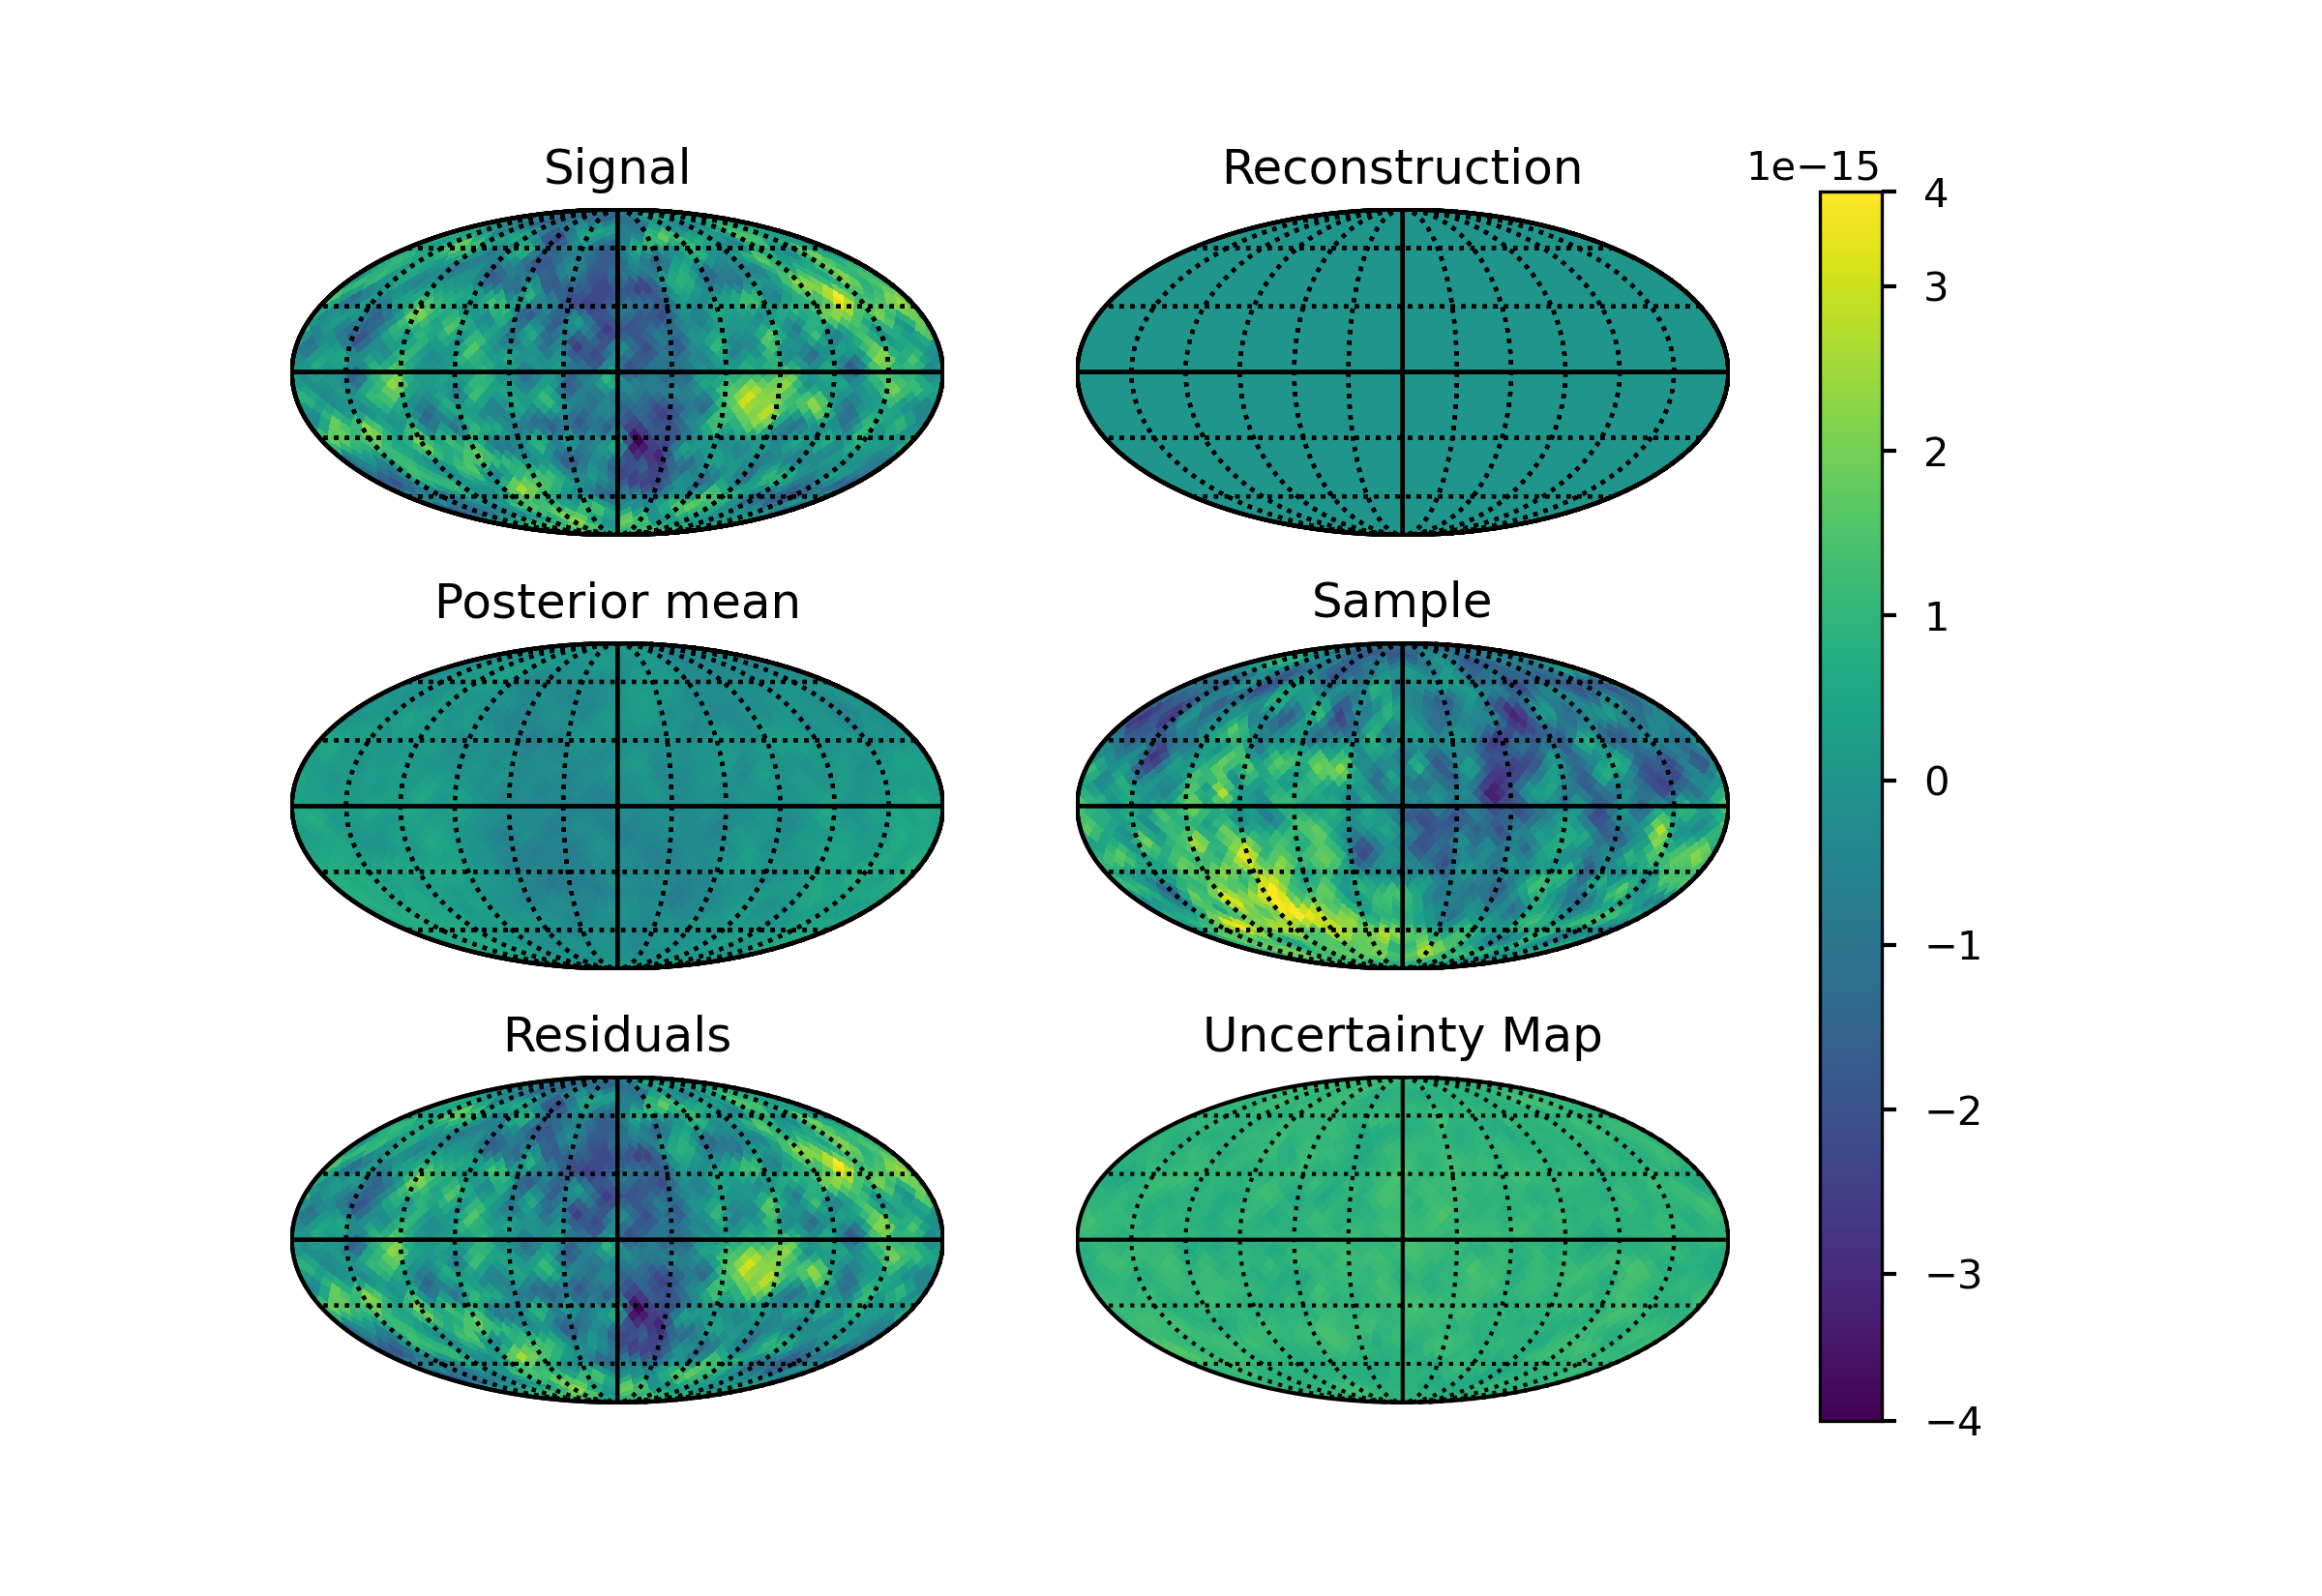
\includegraphics[width=\linewidth]{Images/6plot_cosmo_900Hz_2D.png}}
    \caption[Reconstruction of the CGWB at 900 Hertz on a sky map using the {\tt NIFTy} code.]{Reconstruction of the CGWB at 900 Hertz on a sky map using the {\tt NIFTy} code. The data on top is generated from the signal which is a realisation of the input power spectrum. The posterior mean is calculated using a Wiener filter. A sample of this is drawn randomly. The residuals represent the difference between signal and reconstruction from the first row. The uncertainty map shows the calculated errors on the reconstruction.}
    \label{sky_maps_cosmo}
\end{figure}

In Fig.\ref{sky_maps_cosmo} it is visible that the data is much noisier than the signal computed from the cosmological power spectrum. The reconstruction is not possible, thus the reconstructed sky map and the posterior mean are near zero. The sample drawn from the posterior mean does not resemble the signal and the uncertainty map averages much higher than the reconstruction. 

\begin{figure}
    \centering
    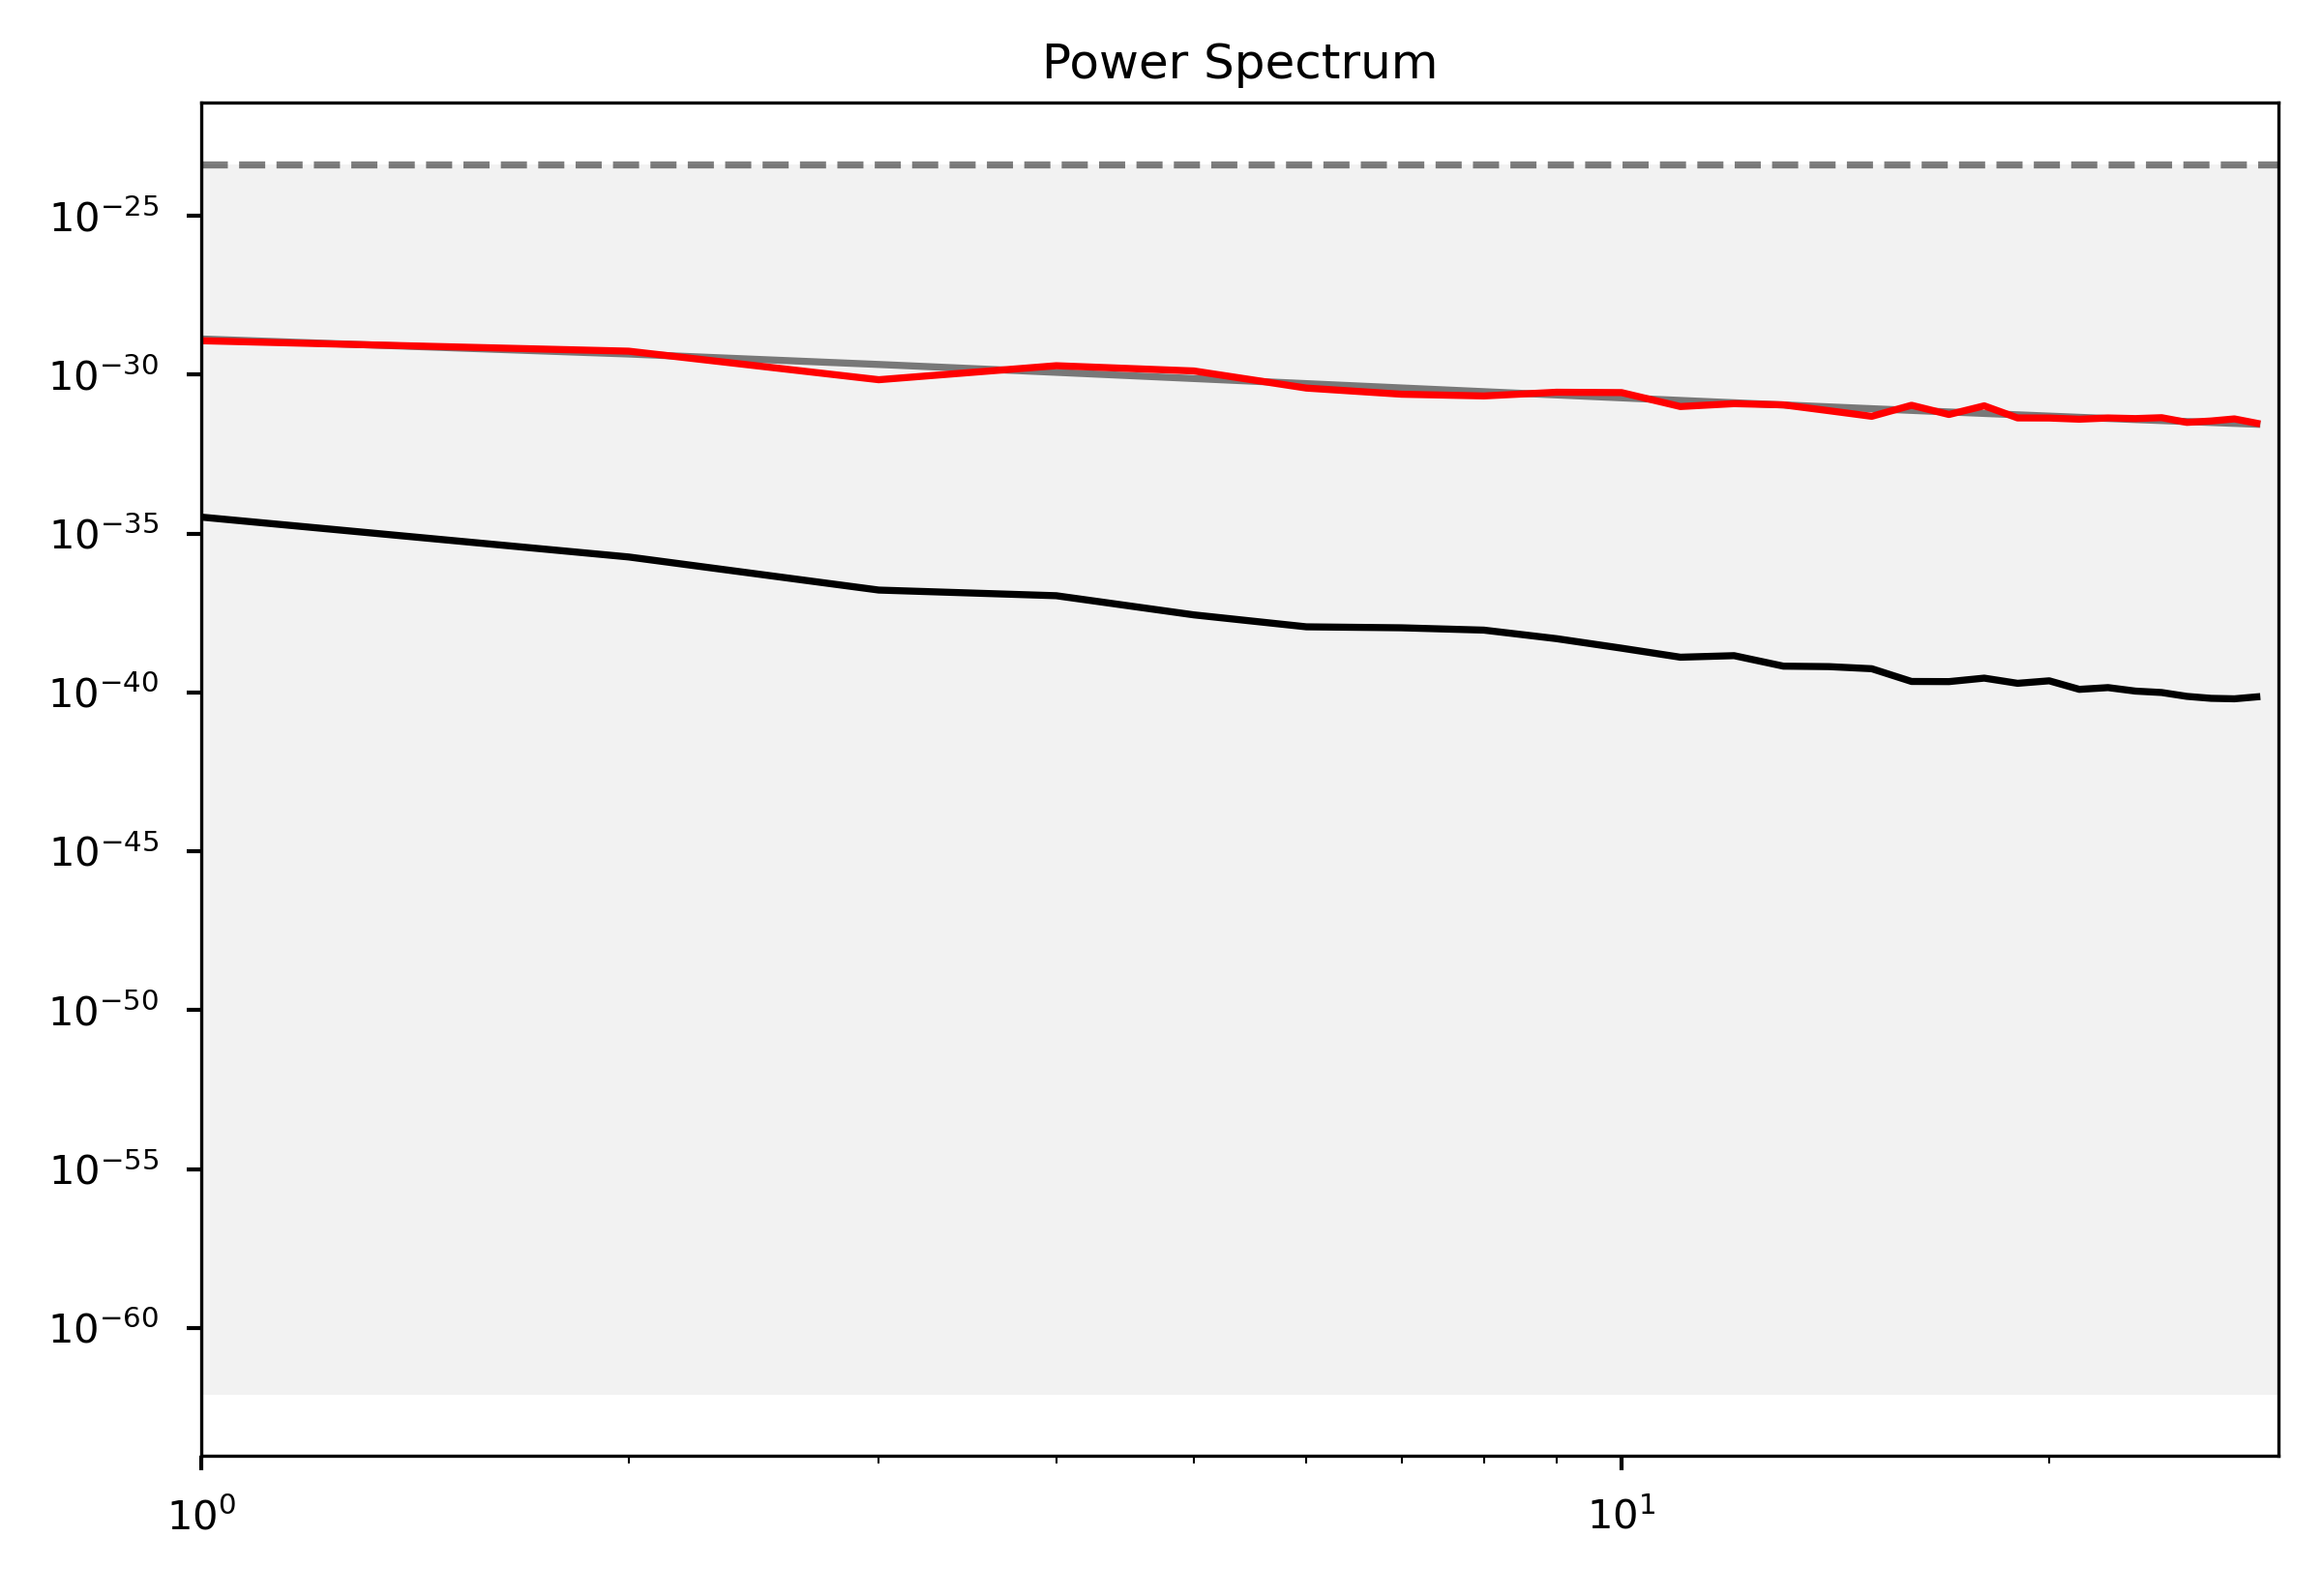
\includegraphics[width=0.8\linewidth]{Images/power_spectrum_cosmo_900Hz_2D.png}
    \caption[The power spectra of the CGWB separation at 900 Hertz.]{The power spectra of the CGWB separation at 900 Hertz. The input power spectrum is shown in grey, the signal realisation in red and the reconstruction using IFT in black.}
    \label{cosmo_power_spectrum_nifty}
\end{figure} 

Looking at the power spectrum in Fig. \ref{cosmo_power_spectrum_nifty}, we see that the noise level is roughly five orders of magnitude higher than the input and signal. Like for the AGWB at 100 Hertz, the reconstruction is much lower than the signal, because it is filtered out together with the noise.